\chapter{生体データを用いたコンテンツへの重畳提示システム}

\thispagestyle{myheadings}

本章では生体データを使いコンテンツに重畳提示する手法について述べる.
図\ref{systemall}に研究の全体像を示す.
システムの流れは,1:コンテンツを視聴しているときの生体データを取得する.
2:生体データをコンテンツ毎に収集する.
3:集めた生体データから盛り上がっている箇所を推定し抜き出す.
4:抜き出したデータを基にコンテンツに重畳提示するといった構成である.

\begin{figure}[H]
    \centering
    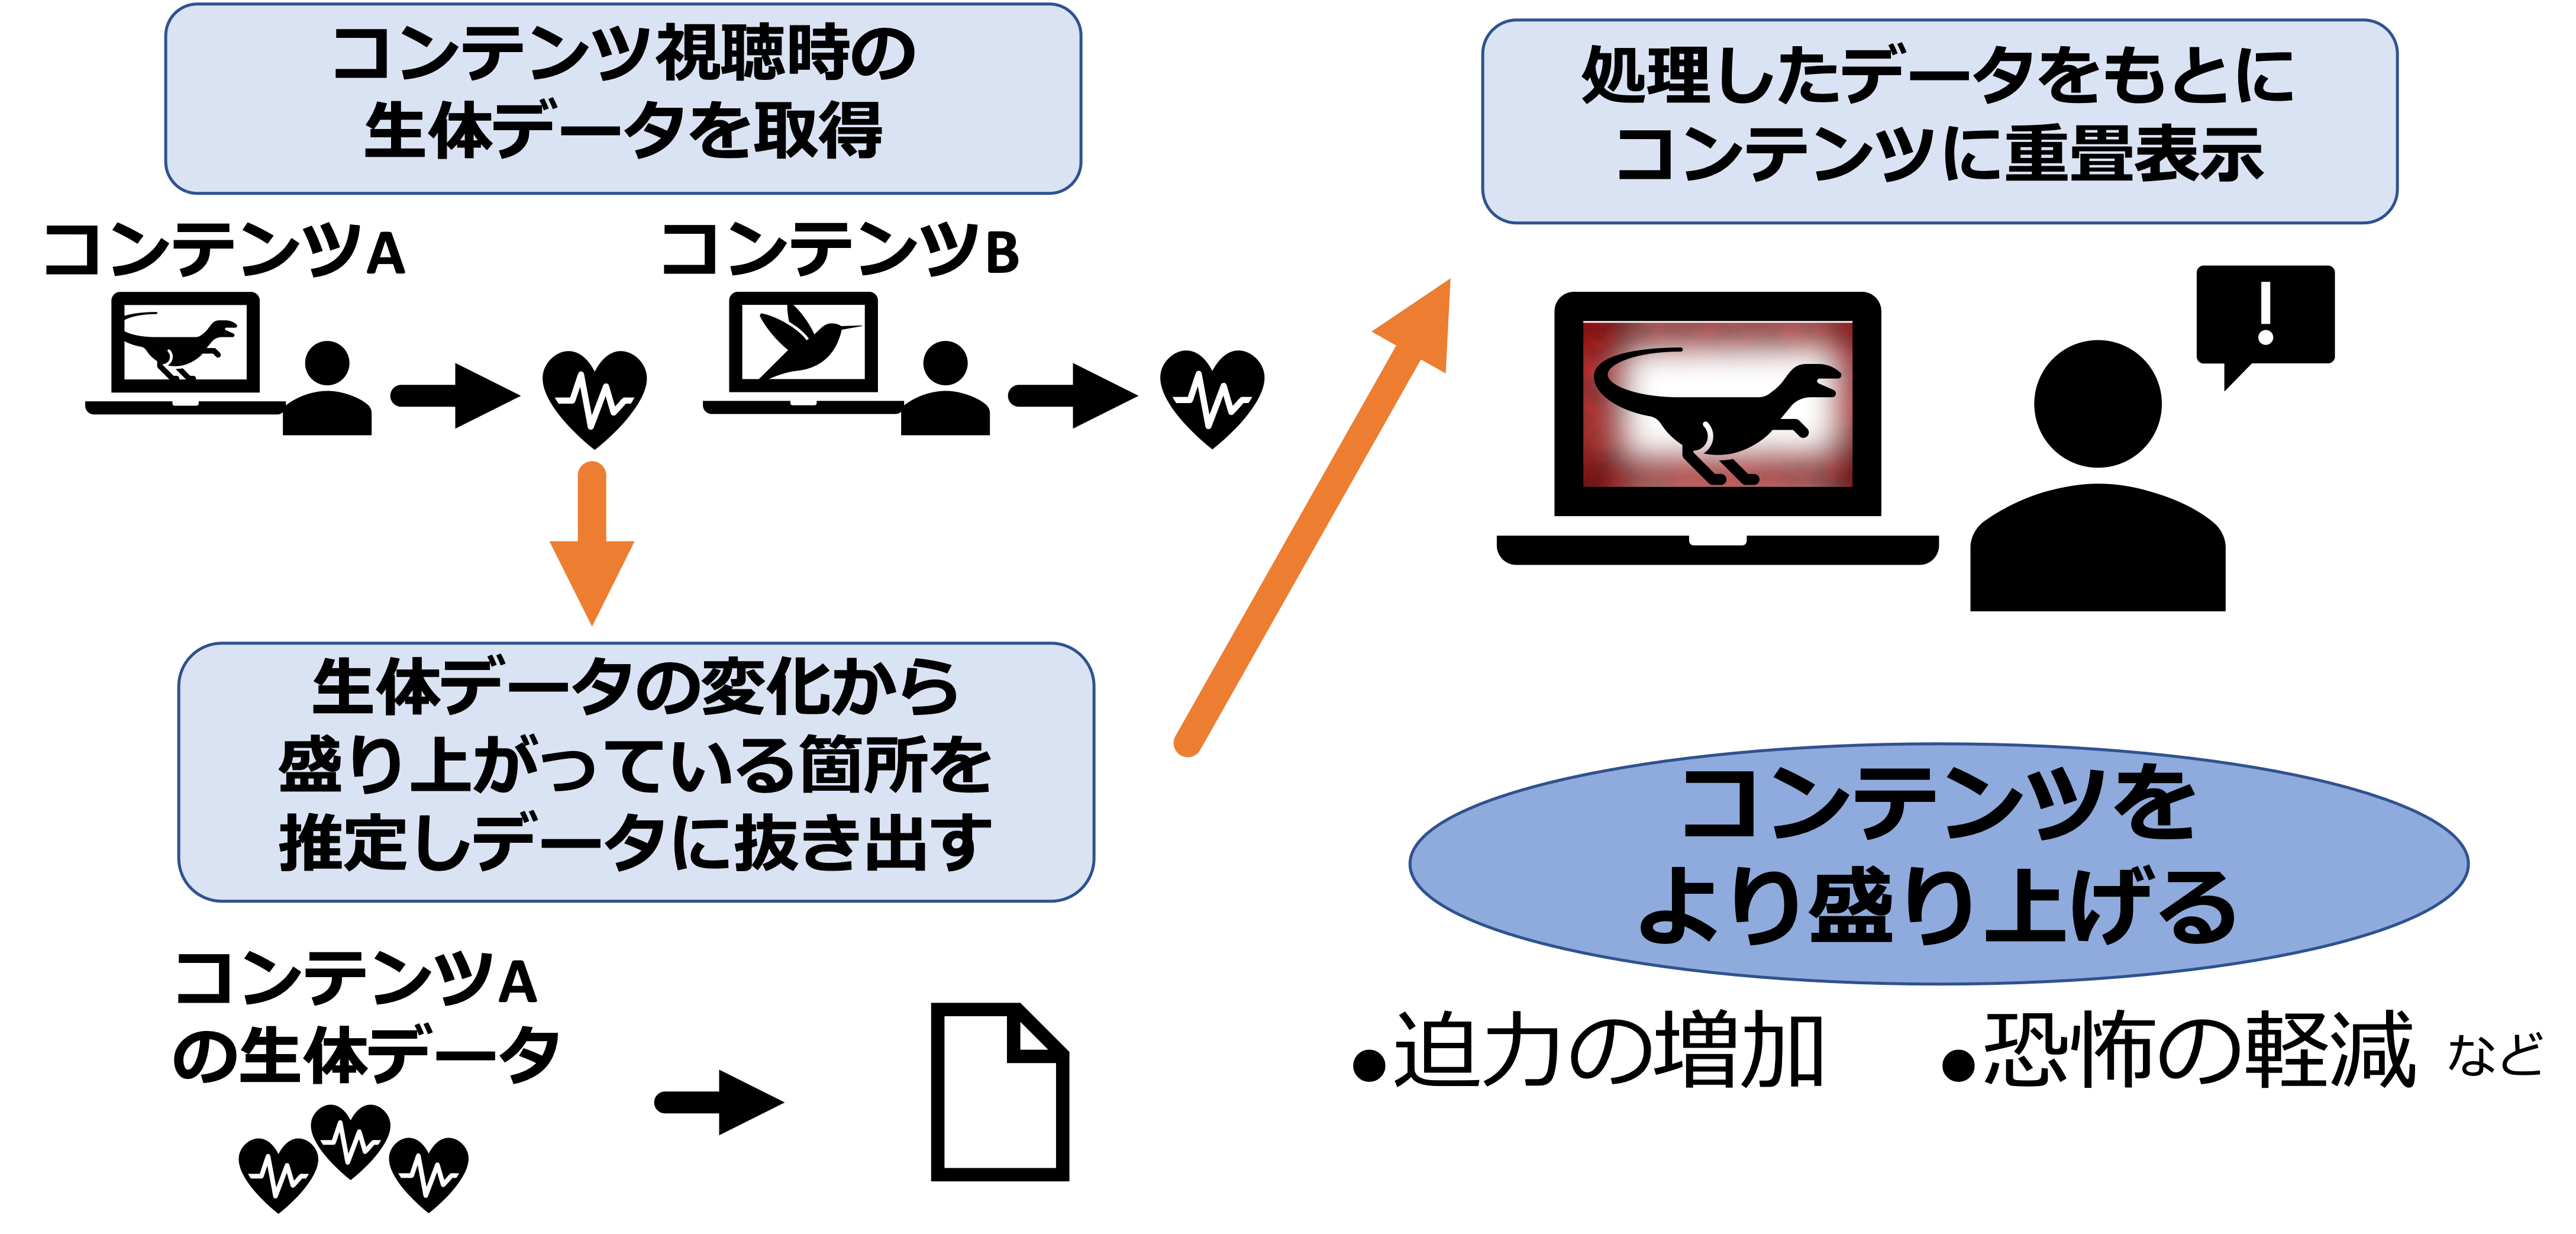
\includegraphics[width=15cm]{images/chapter3/allsysytem.png}
    \caption{システム全体図}
    \label{systemall}
\end{figure}



コンテンツ視聴時に生体データを利用するとコンテンツに対し視聴者が興奮している箇所を推定できる.
本研究ではコンテンツの盛り上がっている箇所を複数人で共有する.
コンテンツのどの箇所で視聴者が盛り上がっていたのかを生体データを使って推定する.
コンテンツにエフェクトを重畳すると(以下,重畳提示),コンテンツに対し抱いた感情をエフェクトという形で可視化できる.
これによってコンテンツに迫力や臨場感を増幅できる.
そのため本研究ではコンテンツ視聴時の生体データを取得し,コンテンツにエフェクトを重畳するシステムの開発を行う.

コンテンツを視聴している時の生体データについて述べる.
収集する生体データとして目の動きに注目したり,額から出る汗の量でコンテンツ視聴時の興奮度を測る方法などが考えられる.
% 収集する生体データによってコンテンツに対する盛り上がり方を色々な目線で計測するのが可能である.
生体データは目の動きや心拍数など多様な種類がある,
そのため視聴するコンテンツによって適した生体データを取得する.
コンテンツには動画や電子書籍などのデジタルコンテンツと本や新聞紙などのアナログコンテンツがある.
本研究のシステムではYouTubeなどを視聴している時の生体データの収集だけでなく,新聞紙や本を読んでいる時も盛り上がりポイントを計測するのが可能である.
例として新聞紙を読んでいる時,生体データとして額から出る汗や目の動きなどでは正確に盛り上がるポイントを見つけ出せない.
新聞紙を読んでいる時は心拍数を使い,面白いと感じる記事を読んでいるときの心拍数を計測するなどコンテンツに合わせた生体データを取得する.
またTwitterやInstagram,Facebook,TiktokなどのSNSコンテンツを閲覧している時にも使用できる.

本研究の重畳提示の手法について述べる.
コンテンツへの重畳提示の手法としては音を追加したり,画面にエフェクトを表示させる,デバイスを振動させるなどさまざまである.
一部のコンテンツには3Dや4DXの映像といった付加効果のついたコンテンツがある.
しかしこれらの付加効果は全てのコンテンツに対応しているわけではない.
本研究は生体データを収集すれば自宅でも好きなコンテンツに対し映像体験が可能になる.
例として本を読んでいる時の重畳手法は,徐々に部屋を暗くしたり雑音をはじめの方は流していて盛り上がるポイントが来たら無音にするなど集中しやすい環境に近づけられる.
その他にも音楽を聴いているときはサビにかけてボリュームを上げビートに合わせてデバイスを振動させライブ会場のようなワクワクが体験できたり,スマートフォンで車のレースゲームをしている時には風を送りゲームに没入感を加えられる.


\section{本研究のシステム構成}
本研究のシステムは,生体データの測定器,収集した生体データを管理するサーバ(以下,サーバ),重畳提示を行うデスクトップアプリケーション(以下,重畳提示アプリ)で構成される.
本システムは映画を見ている時の心拍数をスマートウォッチを使って計測し,取得した心拍データをスマートウォッチからサーバにアップロードする.
アップロードされた心拍データから心拍数が上昇している箇所のみを抜き出す.
その心拍上昇箇所のみの心拍データを基に映画画面に直接画面を囲うようなエフェクトを重畳するという流れになっている.

まず,生体データの測定器としてスマートウォッチを採用した.
理由として近年スマートウォッチは普及しており,誰でも気軽に生体データを取得できるからである(図\ref{watchfukyuu}).
本研究でスマートウォッチは,心拍測定機能が搭載されたTicWatchE3を使用した(図\ref{watche3}).
本研究におけるコンテンツは,研究の提案段階として映画の視聴に限定した.
コロナ禍により自宅で映画を視聴する機会が増えたと考えられるためである.
また一般的に映画は見せ場となるシーンが用意されている場合が多く,盛り上がるポイントが判定しやすいと予想した.
映画を視聴している時の生体データとして,スマートウォッチを使用して心拍数を計測する.
映画を視聴している時は心拍数が頻繁に変化し生体データとして適していると考えたためである.

次に,ユーザごと計測した心拍データはサーバに収集される.
収集された心拍データは映画毎に分類し,蓄積する.
映画毎に蓄積された心拍データは,心拍数が上昇している箇所をそれぞれ抽出する(以下,抽出データ).
心拍数が上昇している箇所は映画が盛り上がっている部分と予想できるためである.
複数の抽出データを基に盛り上がりの特徴量を算出する.
盛り上がりの特徴量とは,映画の時間毎に心拍数の上昇しやすい箇所を算出したものである.
これは重畳提示を行うためのデータになる.

重畳提示アプリを用いて,映画に直接エフェクトを重畳する.
まず重畳提示アプリは,視聴する映画に合わせてサーバから盛り上がりの特徴量を取得する.
取得した盛り上がりの特徴量を基に映画の時間毎に心拍数の上昇しやすい箇所で,映画画面に直接枠を囲うようなエフェクトを重畳する.
映画のジャンルに応じて幾つかのエフェクトを用意した.
ジャンルによって迫力や恐怖といった感情が異なるため,ジャンル毎に適切なエフェクトを重畳するためである.
重畳提示によって映画から得られる迫力や恐怖などの感情を増幅して体験できると考えた.


\begin{figure}[H]
    \centering
    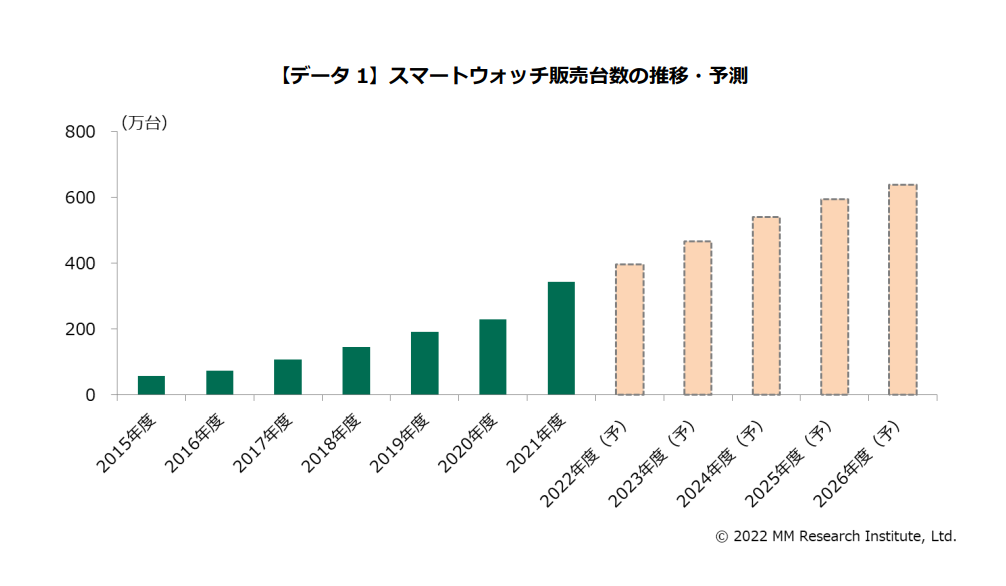
\includegraphics[width=14cm]{images/chapter3/watchreserch.png}
    \caption{スマートウォッチの普及率:2022 MM Research Institute, Ltd.}
    \label{watchfukyuu}
\end{figure}

\begin{figure}[H]
    \centering
    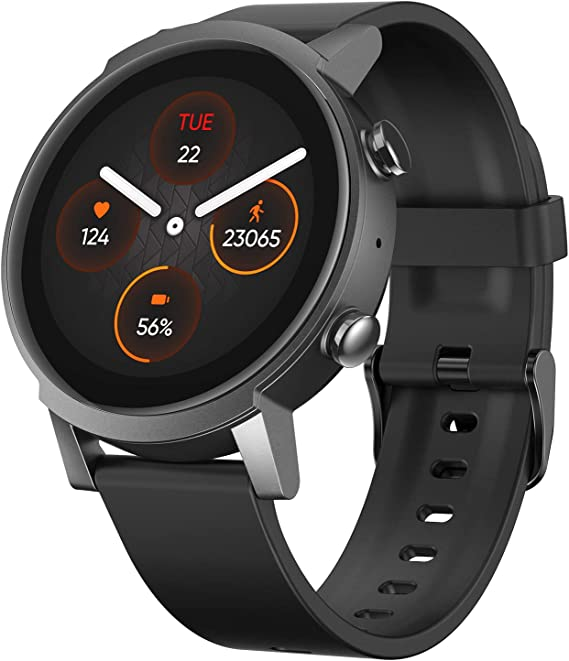
\includegraphics[width=5cm]{images/chapter3/watch.jpg}
    \caption{利用したスマートウォッチ,TicWatchE3}
    \label{watche3}
\end{figure}


\section{心拍データの収集と盛り上がりの特徴量の算出}

本節ではシステムを構成する機能のうち,スマートウォッチを使い心拍データを取得する方法,
収集した心拍データから心拍数が上昇している箇所の抽出方法について述べる.

\subsection{心拍データの収集手法}

心拍データは,映画を視聴している時の心拍数をスマートウォッチを使用して計測する.
本研究では映画を視聴している時の心拍数を計測するため,Android Studioで心拍数が取得できるスマートウォッチ用アプリケーションを作成した.
アプリ画面を図\ref{bpmget}に示す.
センサ取得ボタンを押すと腕につけた時の心拍数を心拍というラベルの下に表示する.
テキストボックスに保存したいファイル名を入力し,記録開始ボタンを押下すると心拍数の記録が開始される.
心拍数を取得中の画面を図\ref{bpmget}の右側に示す.
心拍数の計測を終了する際は,CSV出力ボタンを押下し計測を終了する.
計測した心拍データは計測終了するとCSV形式でサーバに自動的にアップロードされる.

\begin{figure}[tbh]
    \centering
    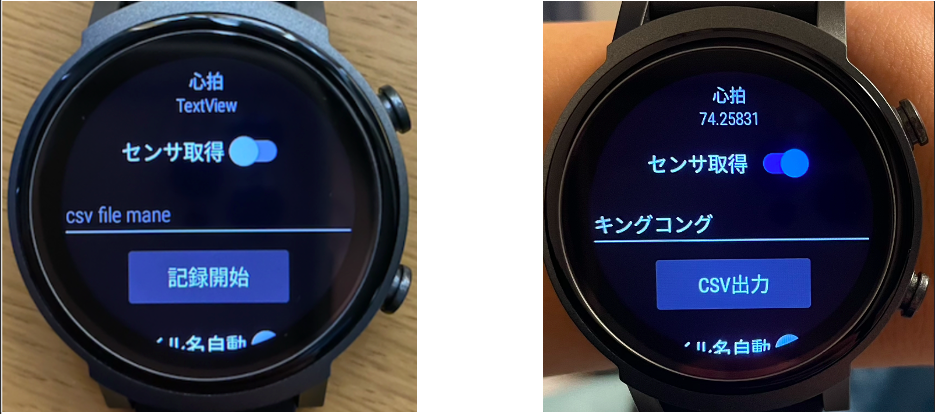
\includegraphics[width=15cm]{images/chapter3/watchgazou.png}
    \caption{心拍数取得画面}
    \label{bpmget}
\end{figure}




\subsection{心拍データと映画の盛り上がり箇所の関連性の分析}

我々は収集した心拍データを観察し,映画の盛り上がり箇所と心拍数の関連性を分析した.
実際に収集した心拍データの一部を図\ref{hitorime},\ref{sannninme},\ref{futarime}に示す.
図\ref{hitorime},\ref{sannninme},\ref{futarime}は,映画「キングコング 髑髏島の巨神」を視聴した3人分のデータである.
また,本映画の見せ場となるシーンは心拍数が上昇すると予想した.
心拍数が上昇すると予想したシーンは需要人物が危機に陥るシーンで,大きく分けて3つある.
1つ目は00:45前後,2つ目は01:30前後,3つ目は01:45前後である.

心拍データは,人ごとに時間毎の心拍数の変動に差異があった.
前述した予想と各サンプルの特徴について言及する.
図\ref{hitorime}のサンプルでは,丸印の箇所で心拍数が上昇しそれ以外は比較的落ち着いている.
丸印の箇所は前述した心拍数が上昇すると予想した時間と一致している.
図\ref{sannninme}のサンプルでは,常に心拍数が上昇と下降を繰り返しており,その変化量は図\ref{hitorime}のサンプルより大きい.
心拍数が上昇すると予想したシーンでは,心拍数の変化は見られなかった.
図\ref{futarime}のサンプルでは,図\ref{hitorime}と同様に心拍数が上昇すると予想したシーンで心拍数が上昇した.
それ以外は上昇と下降を繰り返しており,その変化量は図\ref{hitorime}のサンプルより大きい.
またサンプル毎に映画視聴中の心拍数の中央値には,ばらつきがあった.

\begin{figure}[H]
    \centering
    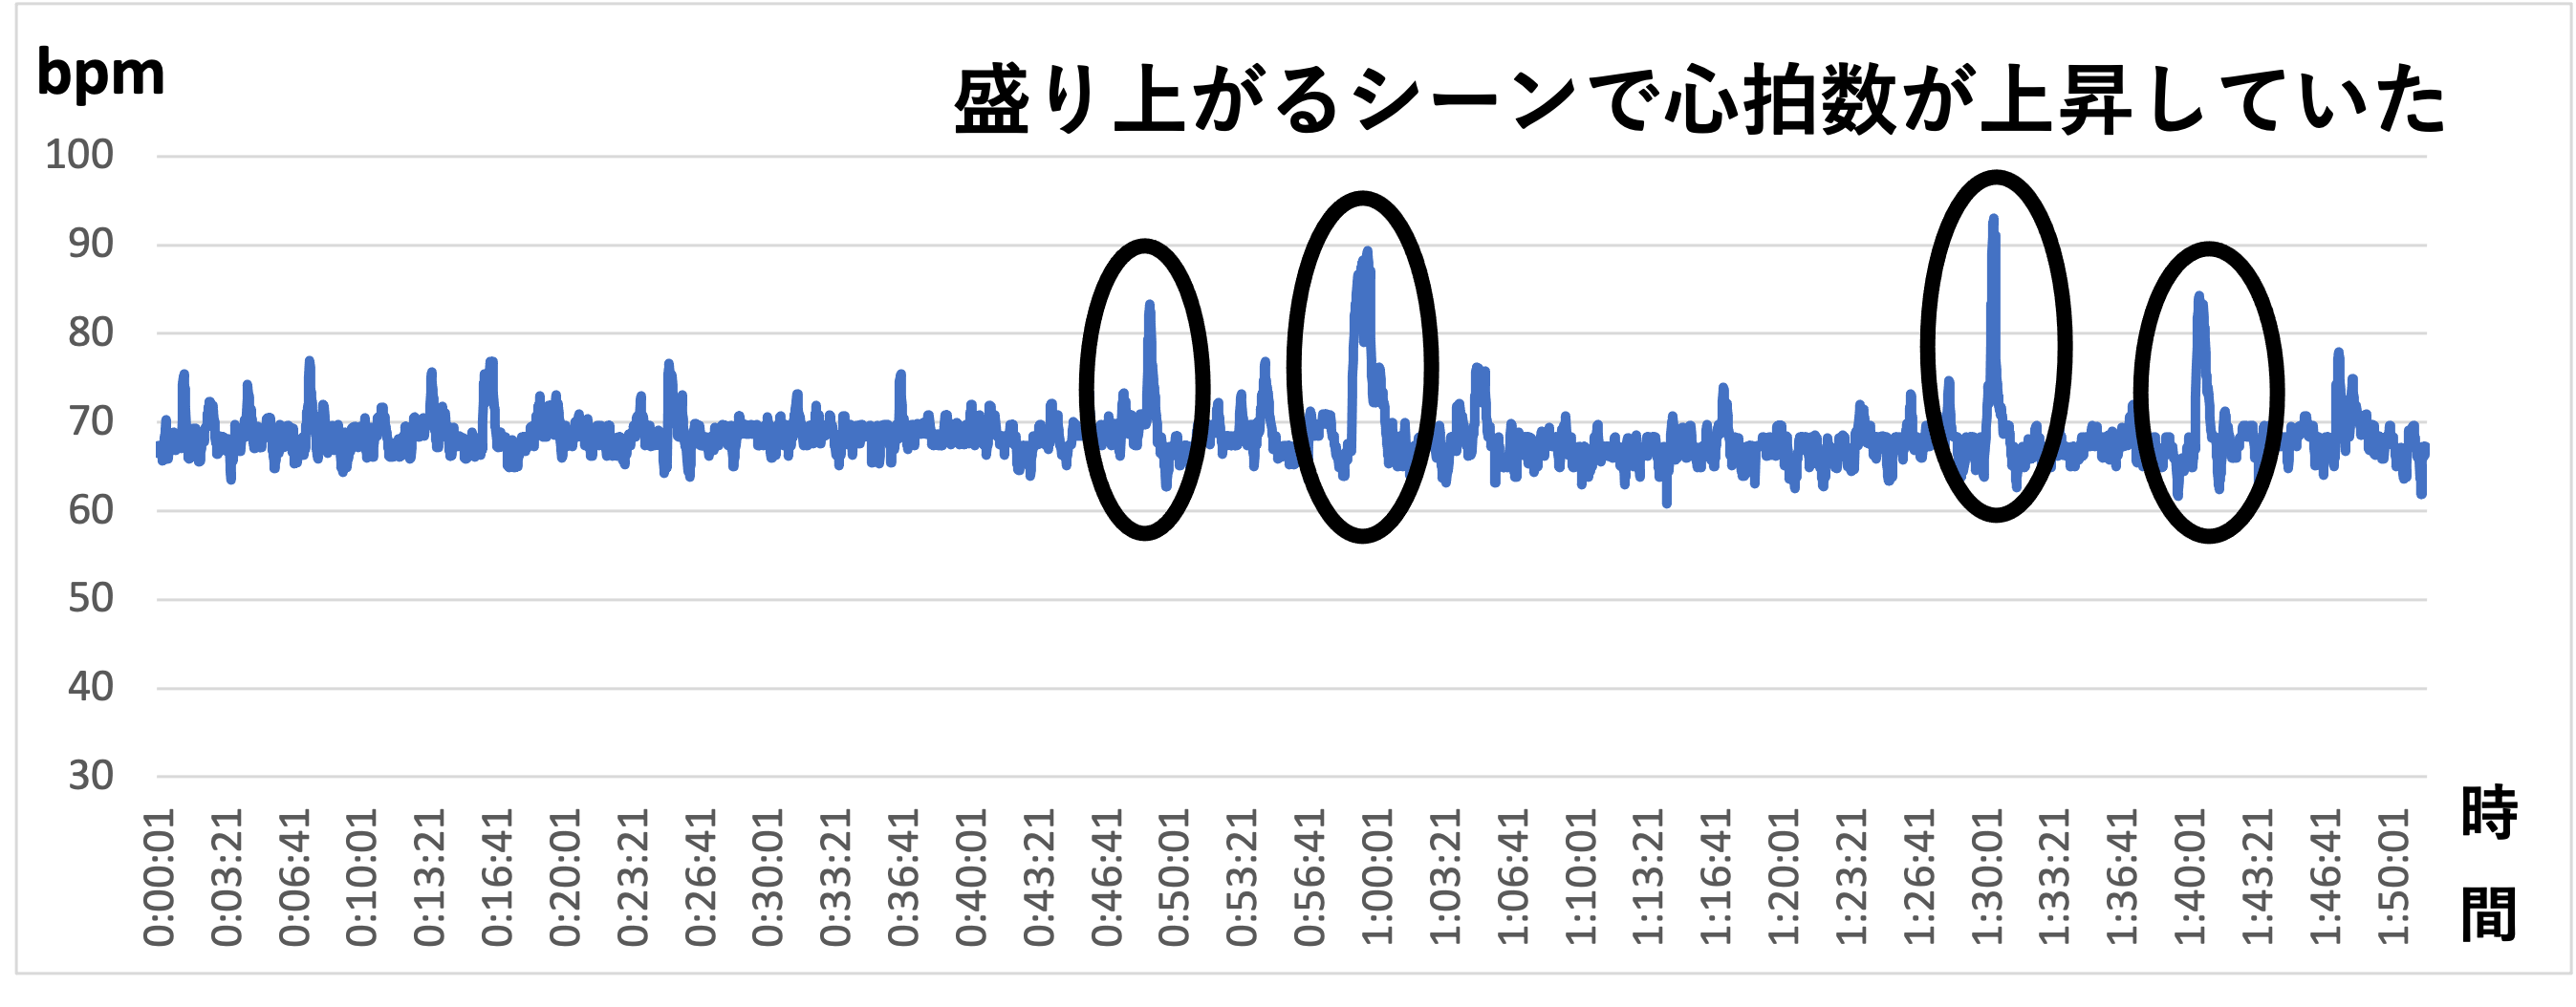
\includegraphics[width=16cm]{images/chapter3/gurafusyuusei.png}
    \caption{キングコングを視聴した時の1人目心拍数のグラフ}
    \label{hitorime}
\end{figure}

\begin{figure}[H]
    \centering
    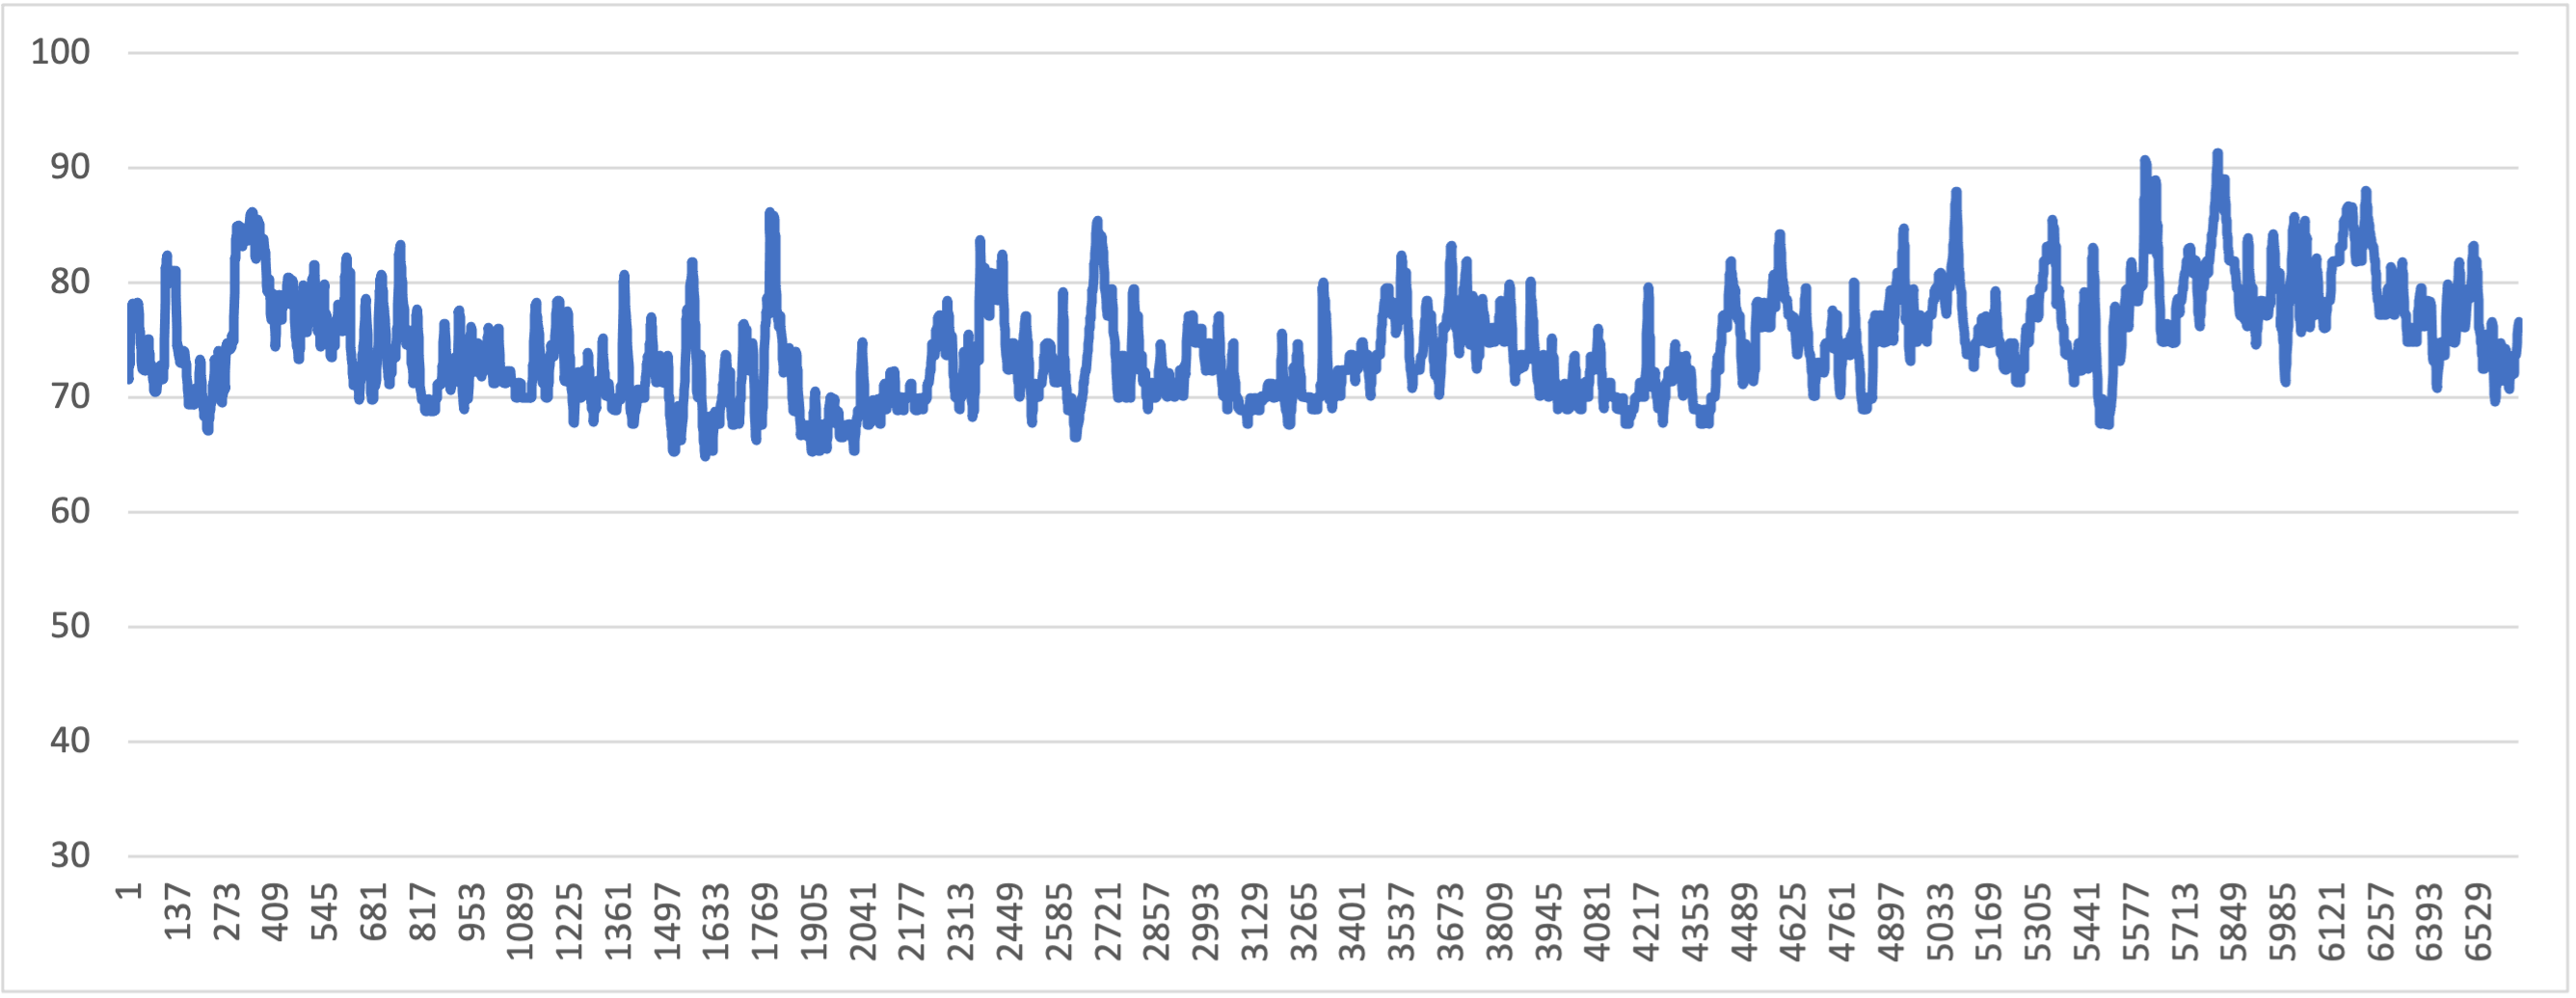
\includegraphics[width=16cm]{images/chapter3/gurafu1.png}
    \caption{キングコングを視聴した時の2人目心拍数のグラフ}
    \label{sannninme}
\end{figure}

\begin{figure}[H]
    \centering
    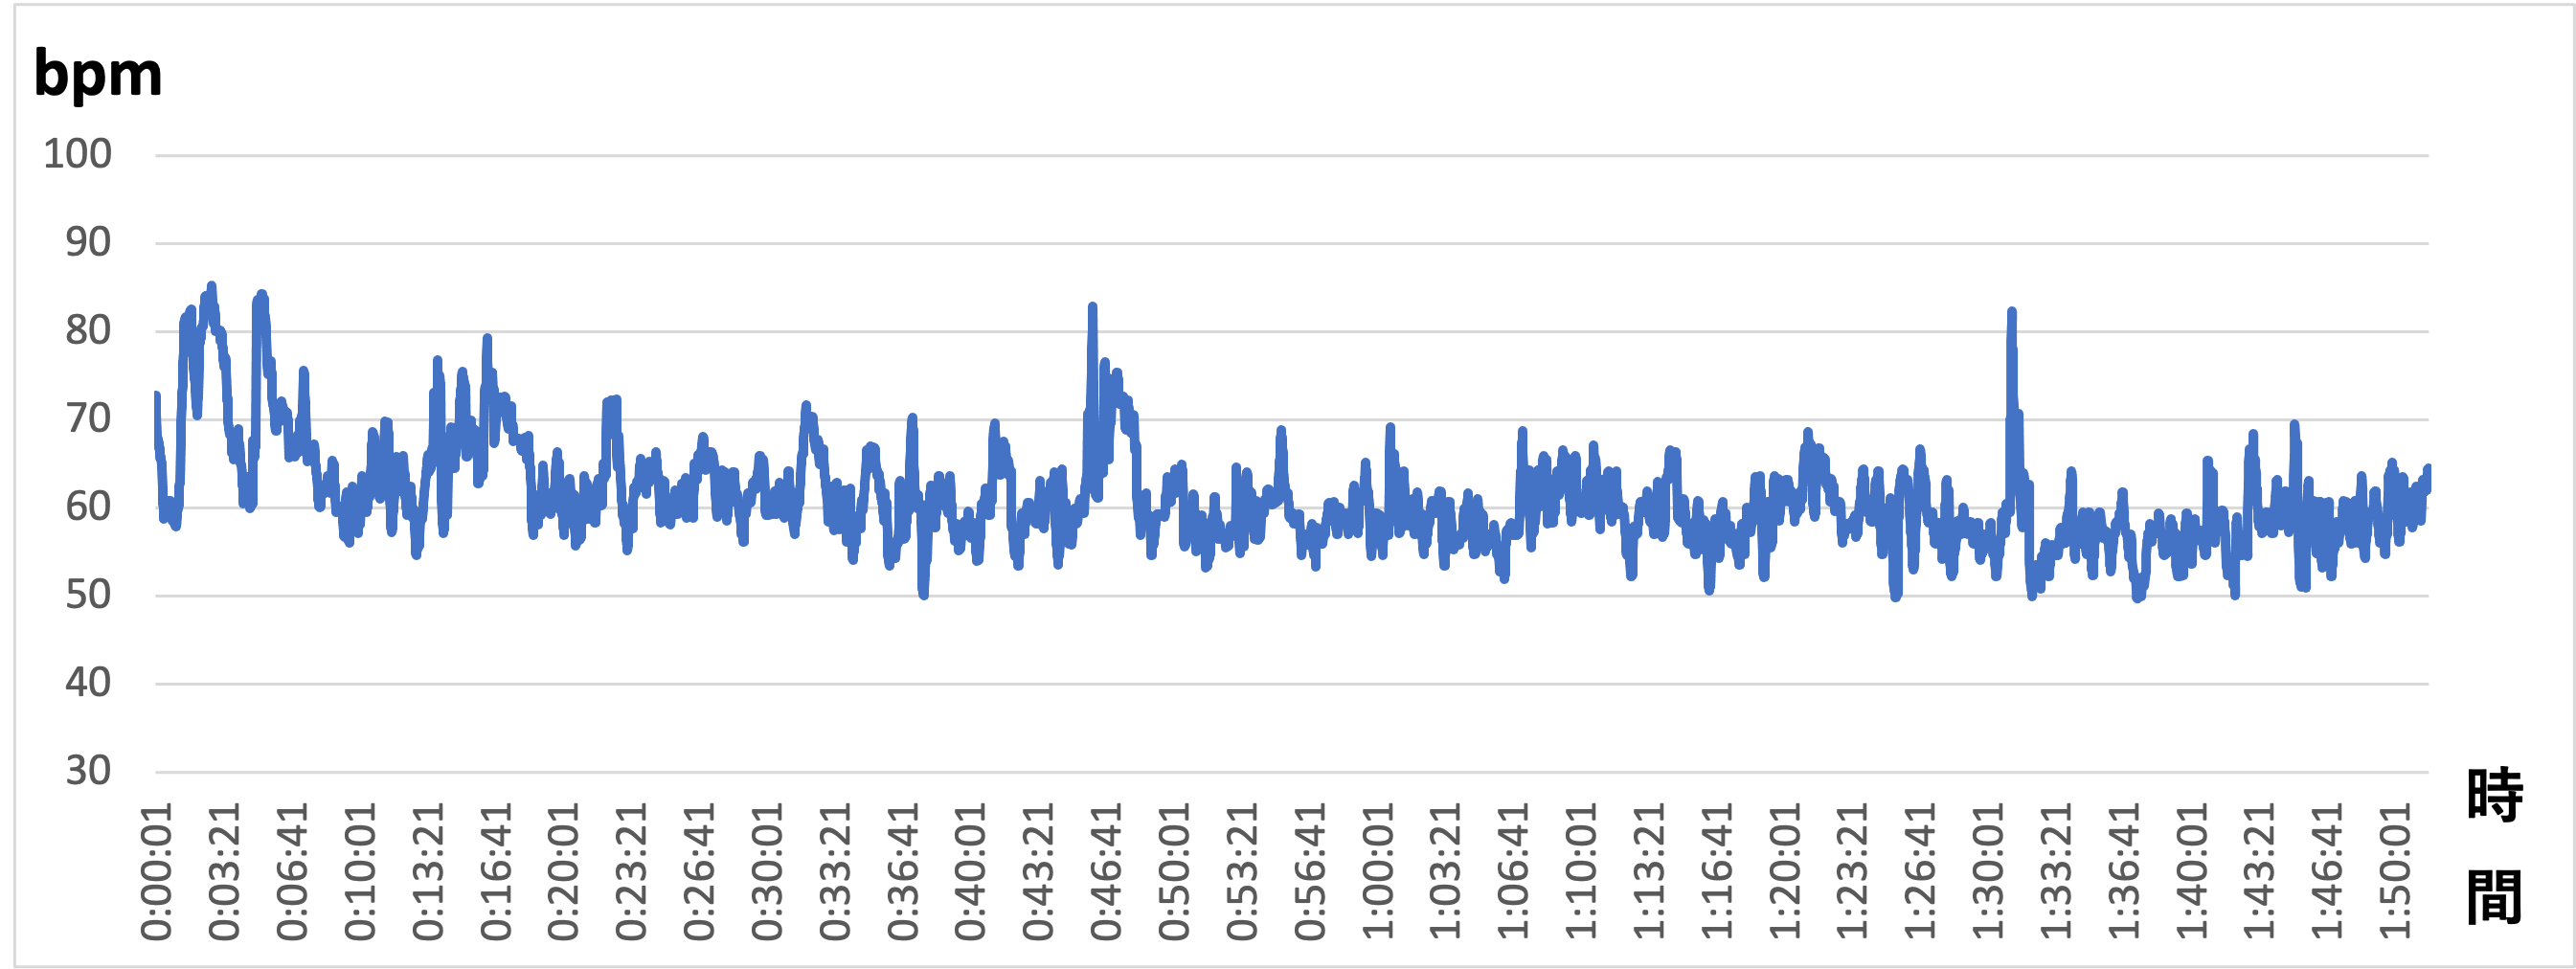
\includegraphics[width=16cm]{images/chapter3/gurafu.png}
    \caption{キングコングを視聴した時の3人目心拍数のグラフ}
    \label{futarime}
\end{figure}

% 心拍数が上昇している箇所を抽出処理するため,
映画の盛り上がるシーンと心拍数の関係性を比較したところ,2つの特徴がわかった.
人により心拍数の中央値はばらつきがあった.
心拍数が大きく上昇している箇所を抽出するには,閾値を設定する必要がある.
しかし人によって心拍数の中央値はばらつきがあるため,一定の閾値による判定は難しい.
閾値は,人ごとに心拍数の中央値が異なるのを考慮して設定する必要がある.
心拍数が上昇すると予想した映画の見せ場となるシーンでは心拍数の上昇が確認できた.
また見せ場となるシーンで心拍数が上昇している時は,全体を通して上昇率が高かった.
よって心拍数と映画が与える感情の変化には比例関係があるとわかった.
% これらより人によって差はあるが映画を視聴している時,見せ場となるシーンでは心拍数が上昇するのが確認できた.



\subsection{心拍数上昇箇所の抽出処理}
収集した心拍データを基に,エフェクト表示に適した形式にするため心拍数が上昇している箇所を抽出するための処理を行う.
収集した心拍数の CSV データをエフェクト表示に適したJSON データに変換する.
まず,サーバから心拍数のCSVデータを取得し心拍数が上昇している箇所の抽出を行う.心拍数上昇箇所の抽出処理の方法を図\ref{bpmupp}に示す.
収集した心拍データを観察し,心拍数が上昇している箇所の抜き出し方法を決定した.人により平均の心拍数はさまざまであったため,
心拍数が上昇している箇所を見つけ出すようまず安静時の心拍数を取得する.安静時の心拍数は,映画を視聴する前の1分間動かない状態で心拍数を計測し取得する.
その安静時の平均心拍数からどれだけ心拍数が上昇したかを抽出する.これにより心拍数が高い人も低い人も同じ抽出処理が可能になる.
表\ref{model}に今回作成したモデルの定義を示す.from toの形式で心拍数が閾値を超えていた時間を示す.
時間は映画が始まってからの経過時間でエフェクト表示するため相対時間にした.今回from toの形式にしたのは,
エフェクトを映画画面に重畳する際にエフェクト表示する時間を心拍数が閾値を超えていた時間の範囲で表示できるようにするためである.
effectlevelで表示するエフェクトを決定する.effectlevelは表\ref{effectlevel}のように心拍数を閾値と比較する.閾値は収集した心拍データを基に設定した.
心拍数の上昇具合で表示するエフェクトを変更するため,1から3までのレベル分けをした.
本研究ではエフェクトを3段階にし心拍数のレベルに応じて表示するエフェクトが変更される.安静時の平均心拍数よりも心拍数が16bpm以上高い時をレベル3,
14bpm以上をレベル2,12bpm 以上をレベル1とする.実際に心拍数上昇箇所の抽出処理をした後のデータを図\ref{bpmsyori}に示す.


\begin{figure}[H]
    \centering
    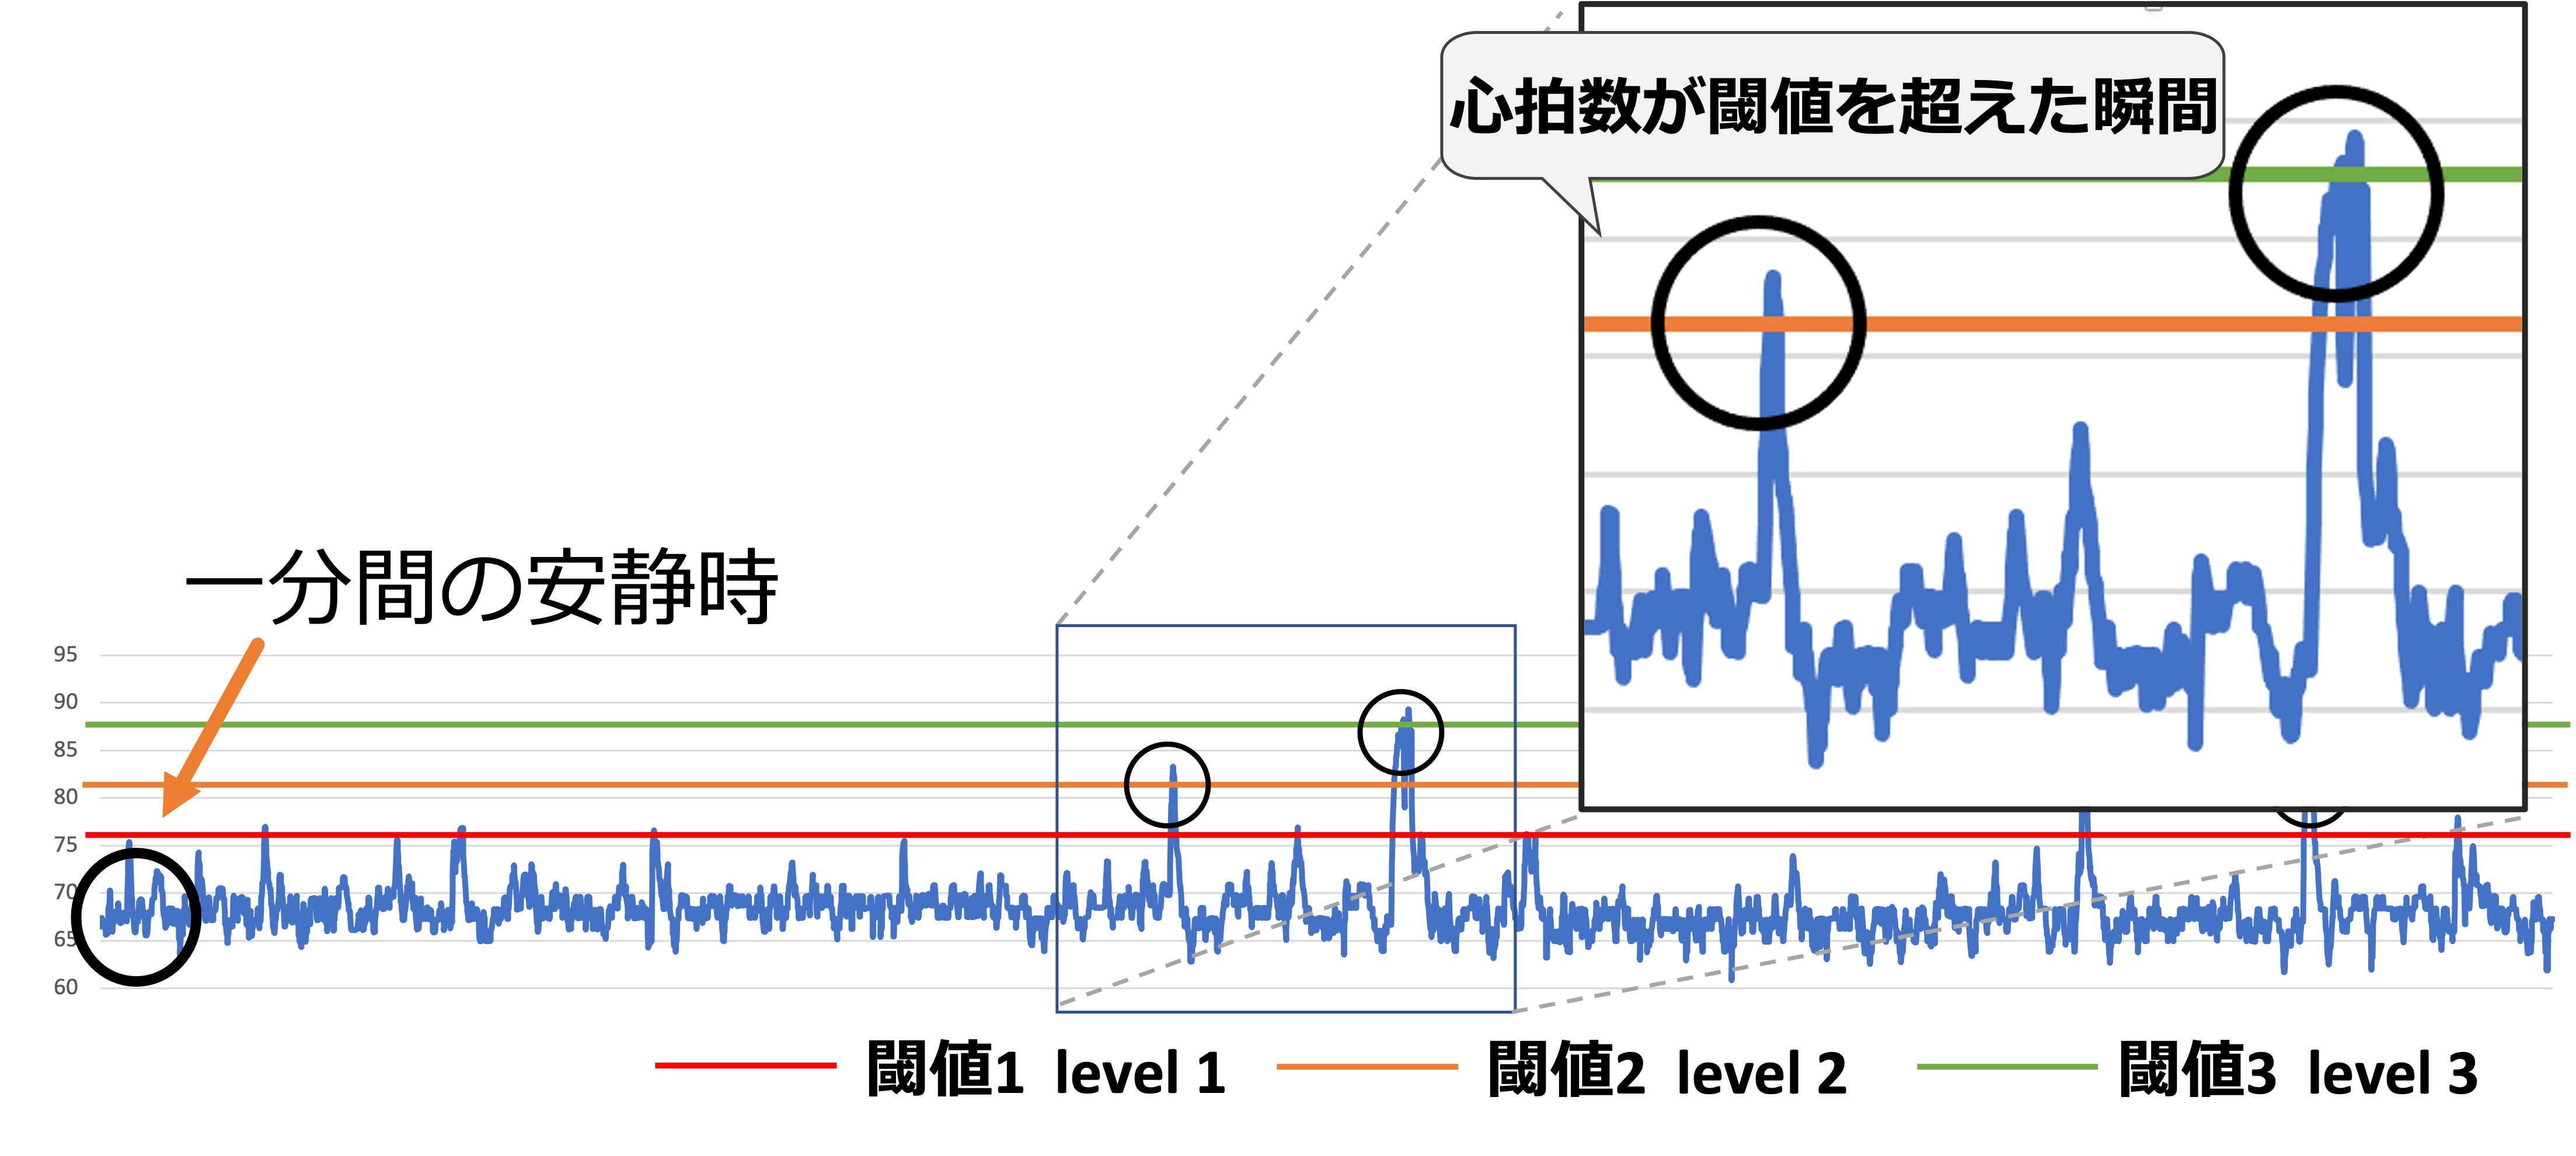
\includegraphics[width=16cm]{images/chapter3/haisyutusyori.png}
    \caption{心拍数上昇箇所の抽出処理}
    \label{bpmupp}
\end{figure}


\begin{table}[htb]
    \begin{center}
        \caption{心拍データのモデルの型定義}
        
        \label{model}
            \begin{tabular}{|c|c|c|} \hline
            	プロパティ & 型 & 説明  \\ \hline \hline
                from & float & 心拍数が閾値を超えた時間 \\ \hline
                to & float & 心拍数が閾値を下回った時間 \\ \hline
                effectlevel & int & 表示するエフェクトのレベル \\ \hline
            \end{tabular}
    \end{center}
\end{table}


\begin{table}[htb]
    \begin{center}
        \caption{閾値設定}
        
        \label{effectlevel}
            \begin{tabular}{|c|c|c|c|} \hline 
            	effectlevel & 1 & 2 & 3  \\ \hline 
                閾値 & 16bpm以上 & 14bpm以上 & 12bpm以上 \\ \hline
            \end{tabular}
    \end{center}
\end{table}



\begin{figure}[H]
    \centering
    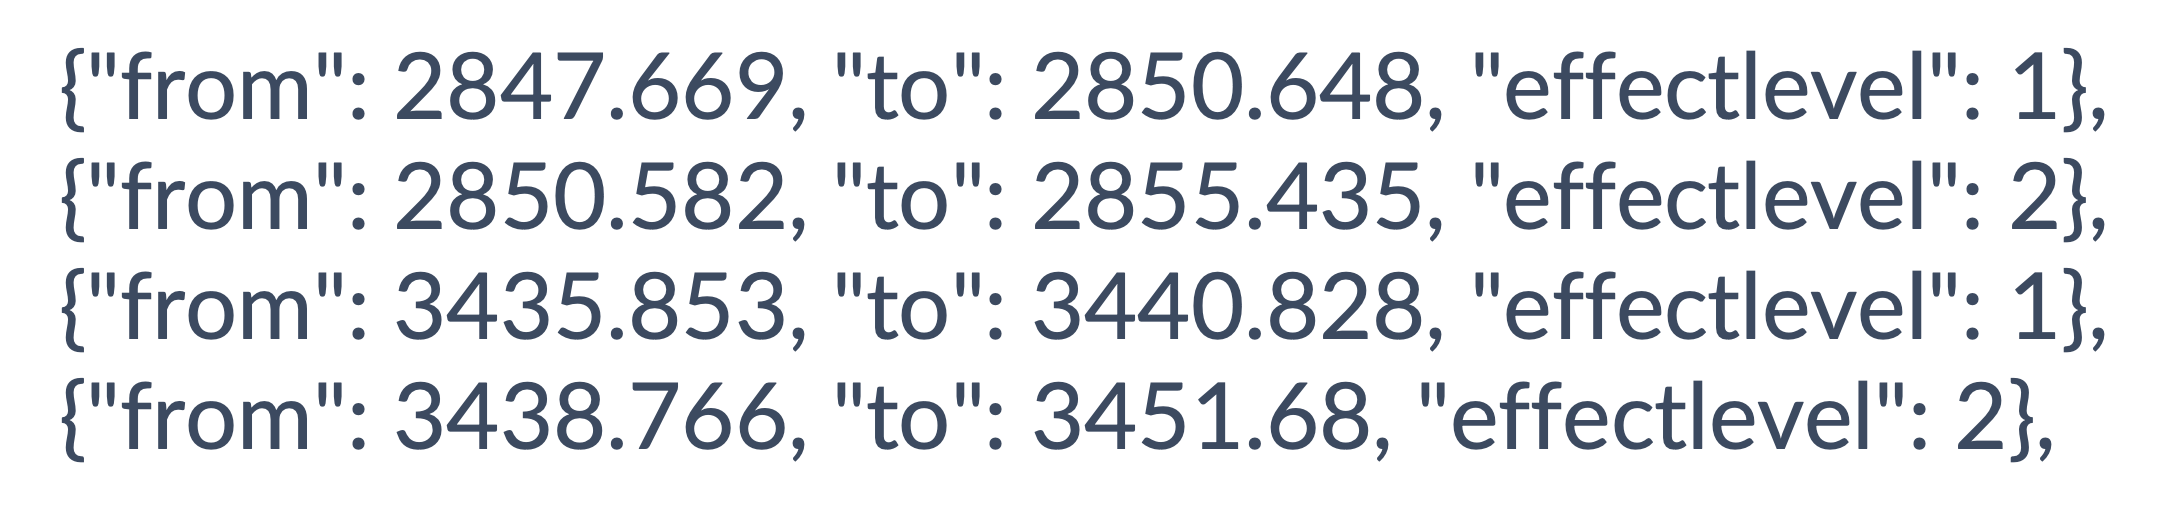
\includegraphics[width=16cm]{images/chapter3/level.png}
    \caption{心拍数上昇箇所の抽出処理をした結果}
    \label{bpmsyori}
\end{figure}


エフェクト表示に適した形式にするため,心拍数上昇箇所の抽出処理したJSONデータを一つのJSONデータにまとめる.
JSONデータの概要を図\ref{gaiyou}に示す.これにより一つのコンテンツに一個のJSONデータが作られる.このデータを使いエフェクトを映画画面に重畳する.

\begin{figure}[H]
    \centering
    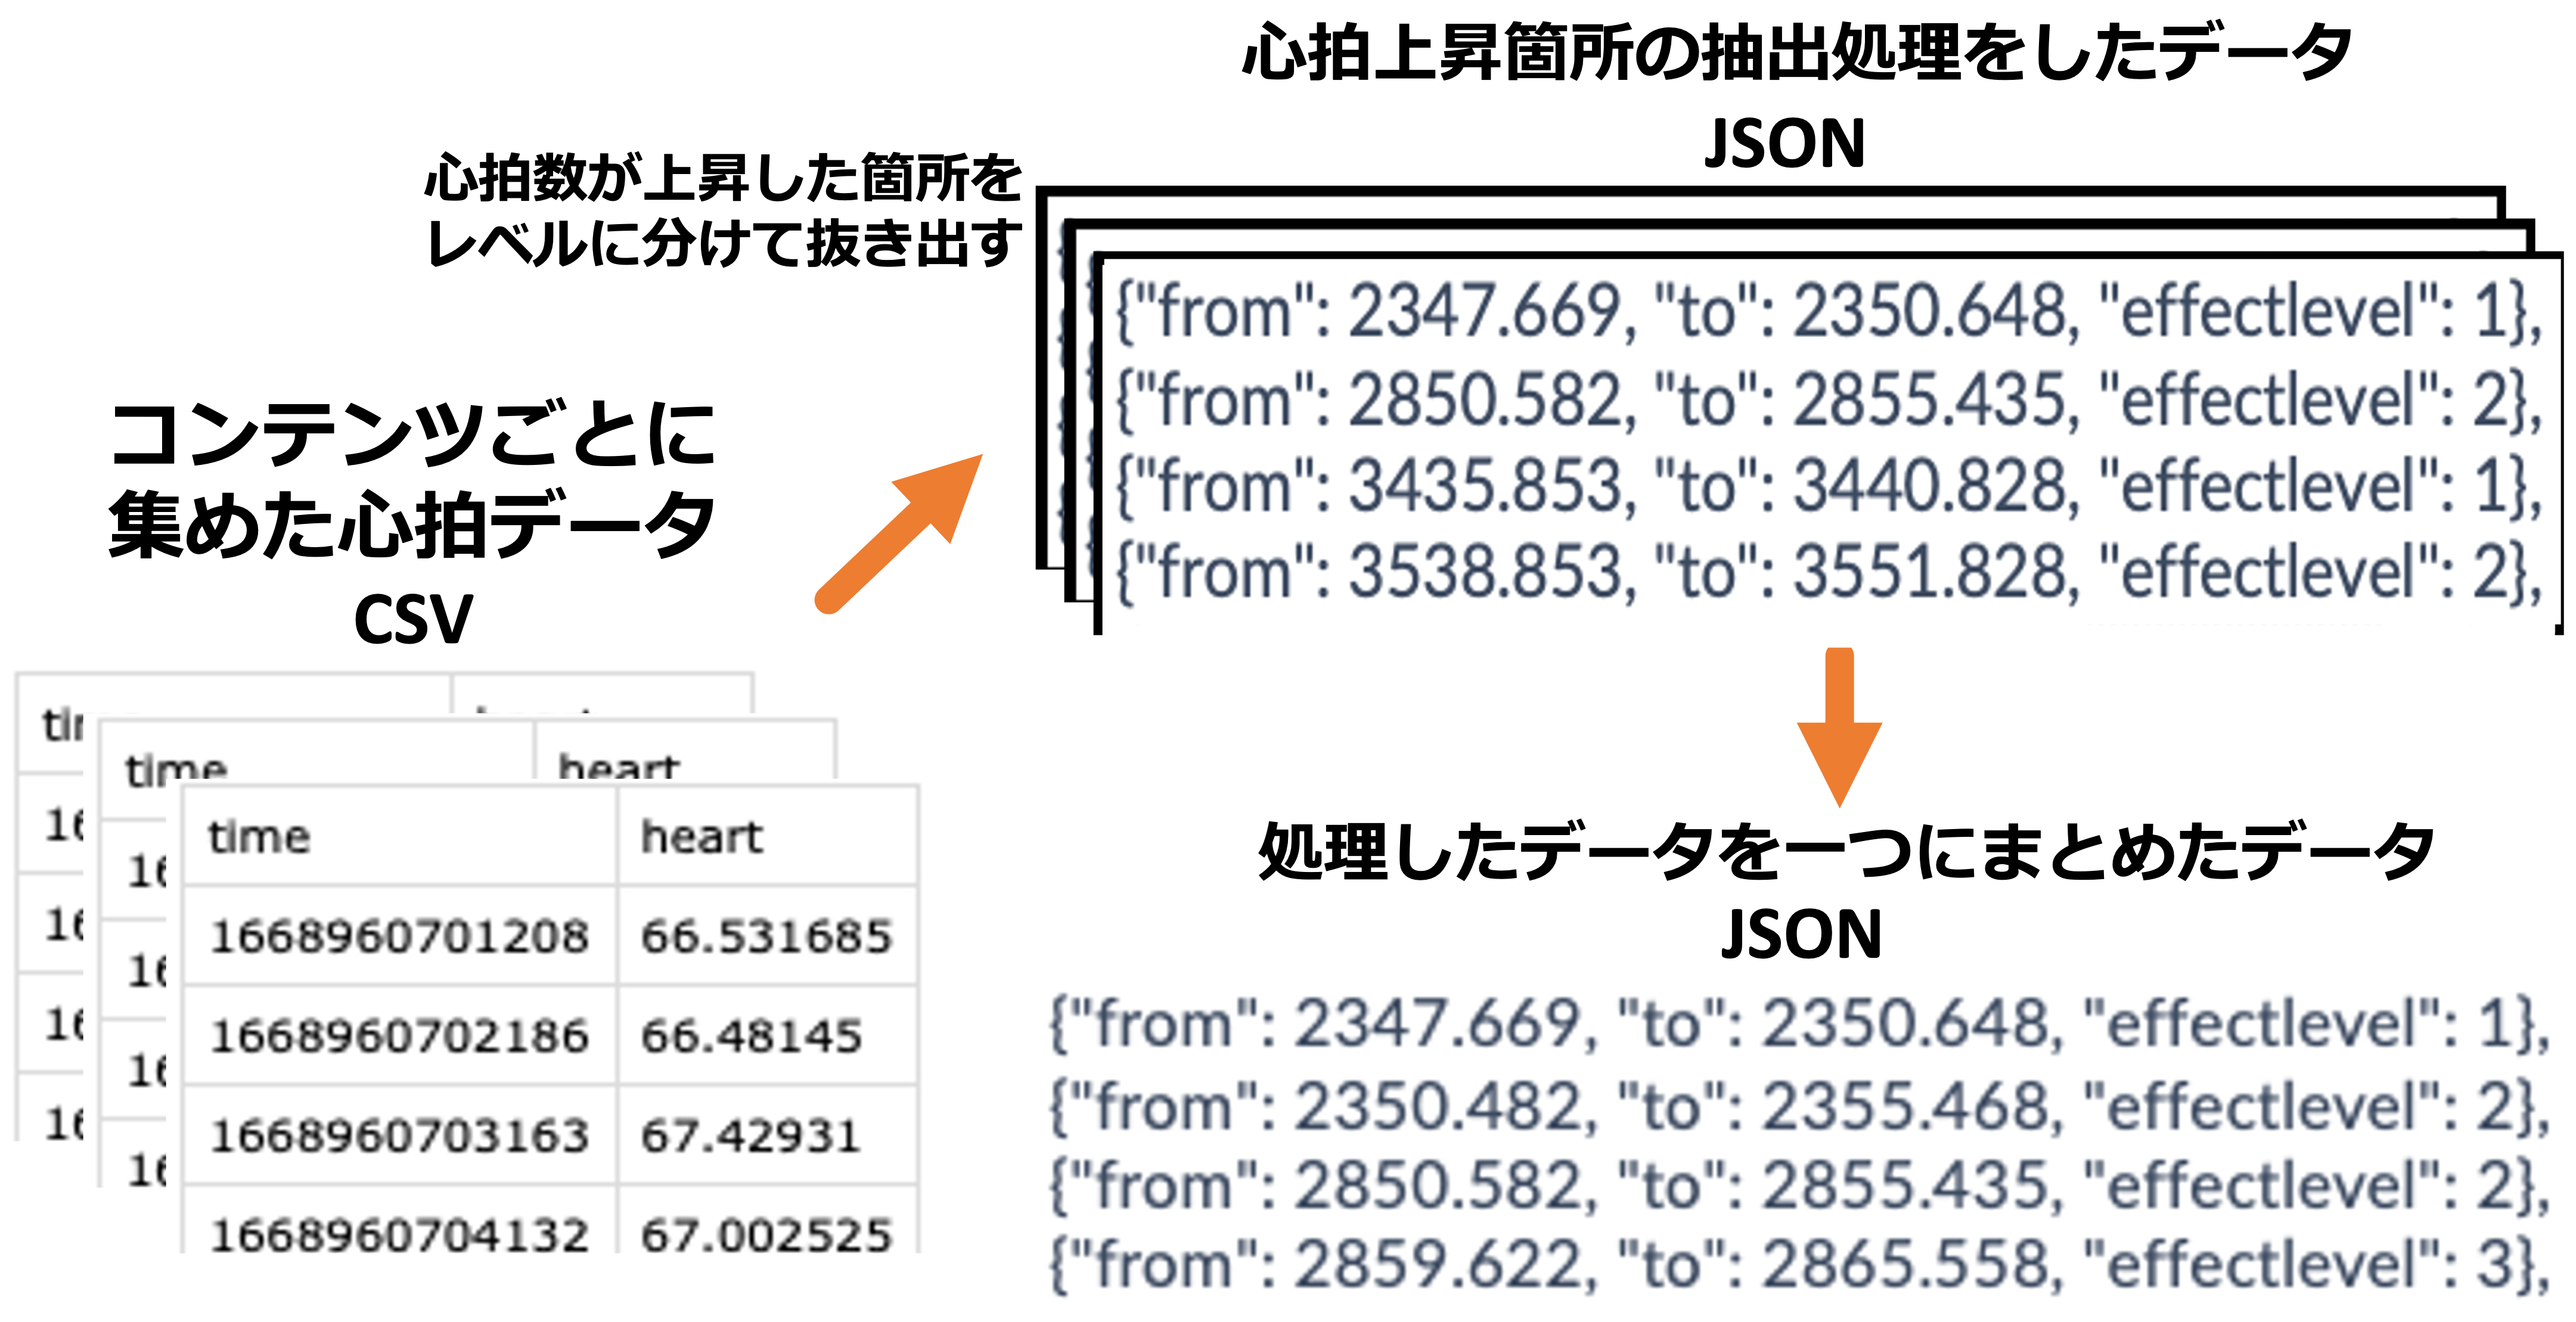
\includegraphics[width=16cm]{images/chapter3/system.png}
    \caption{心拍データの概要図}
    \label{gaiyou}
\end{figure}


\section{重畳提示を行うデスクトップアプリケーション}

 本節では,作成した重畳提示を行うためのデスクトップアプリケーションについて言及する.
 まず作成した重畳提示アプリの設計と構築について,次に実際に重畳するエフェクトについて述べる.

\subsection{重畳提示アプリの設計と構築}

% FIXME: 設計の要件としてこれは入れらる → コンテンツ共有を複数人で行い,個人で重畳提示手法を選択可能にするためである。
% コンテンツ共有とは、視聴している動画に対して過去のユーザの心拍数を基にエフェクト重畳を行うためである。
% 個人で重畳提示手法を選択可能とは、視聴している動画のジャンルごとにエフェクトの種類を個人で選択可能にし、新しい映像効果を与える。

盛り上がりの特徴量を基に,映画に映像効果を付与するデスクトップアプリケーションを構築する.
重畳提示アプリは利用者がコンテンツに没頭しやすいように手軽に利用できる設計を目指した.
重畳提示アプリは,PCを前提に設計する.
スマートフォンは悪意のあるアプリがオーバーレイなどの手段でUIを不明瞭にし,ユーザの意図しない特定のアクションを実行させる可能性があるため.セキュリティが厳重に設定されている.
そのためスマートフォンによる実装はいくつかの特殊な許可をユーザから得る必要がある.
スマートフォンによる実装は,重畳提示アプリとして上記の問題から手軽さが失われてしまうと考えた.
また動画プラットフォームを使用するデバイスとしてテレビが挙げられるが,他システムによる介入が技術的に困難なためPCで実装を行う.
重畳提示アプリをPCで実装するメリットとして,アプリをブラウザのみに対応すれば良い点が挙げられる.
スマートフォンやテレビには,動画プラットフォームごとに独立したアプリケーションが存在する.
この場合,重畳提示アプリはそれぞれのアプリケーションに対応する必要がある.
しかしPC版では,これらのサービスはウェブアプリケーションとして提供されている.
そのため重畳提示アプリはブラウザのみに対応するば,ウェブアプリケーションで提供されるサービスに全て対応できる.

重畳提示アプリは,ウェブ技術を用いてデスクトップアプリケーションを作成できるElectronを用いて構築した.
Electronは,クロスプラットフォームにアプリケーションを作成できるライブラリである.
その為WindowsやmacOSといった,複数のOSに対して一つソースコードで実装が可能である.
Electronを採用した理由は上記のメリットに加え,ウェブ技術を用いて多様なエフェクトを実現できると考えた.
またエフェクトについては\ref{show_effect}項で言及する.

重畳提示を行うには,まず盛り上がりの特徴量をサーバから取得する.
視聴している人の心拍のデータを視聴画面にエフェクト重畳し,
視聴している人に過去のデータの表示,手動でデータ転送を行なった.
視聴している心拍表示をリアルタイムでエフェクト重畳提示できるのが理想だが,
今回は手動でデータ転送を行う方式とした.
本研究は,視聴動画が盛り上がりの特徴量のある際にエフェクト重畳を行なうため,
盛り上がりの特徴量は1から3段階に分けられた.
上記を基にElectronでエフェクトを重畳提示する.
エフェクト提示方法として,Electronを起動,視聴する画面に重畳を行い,視聴する動画を選択提示するエフェクトを選択,Playをクリックしエフェクト重畳が開始する.
その例を図\ref{efectsentaku}に示す.
 
\begin{figure}[H]
   \centering
   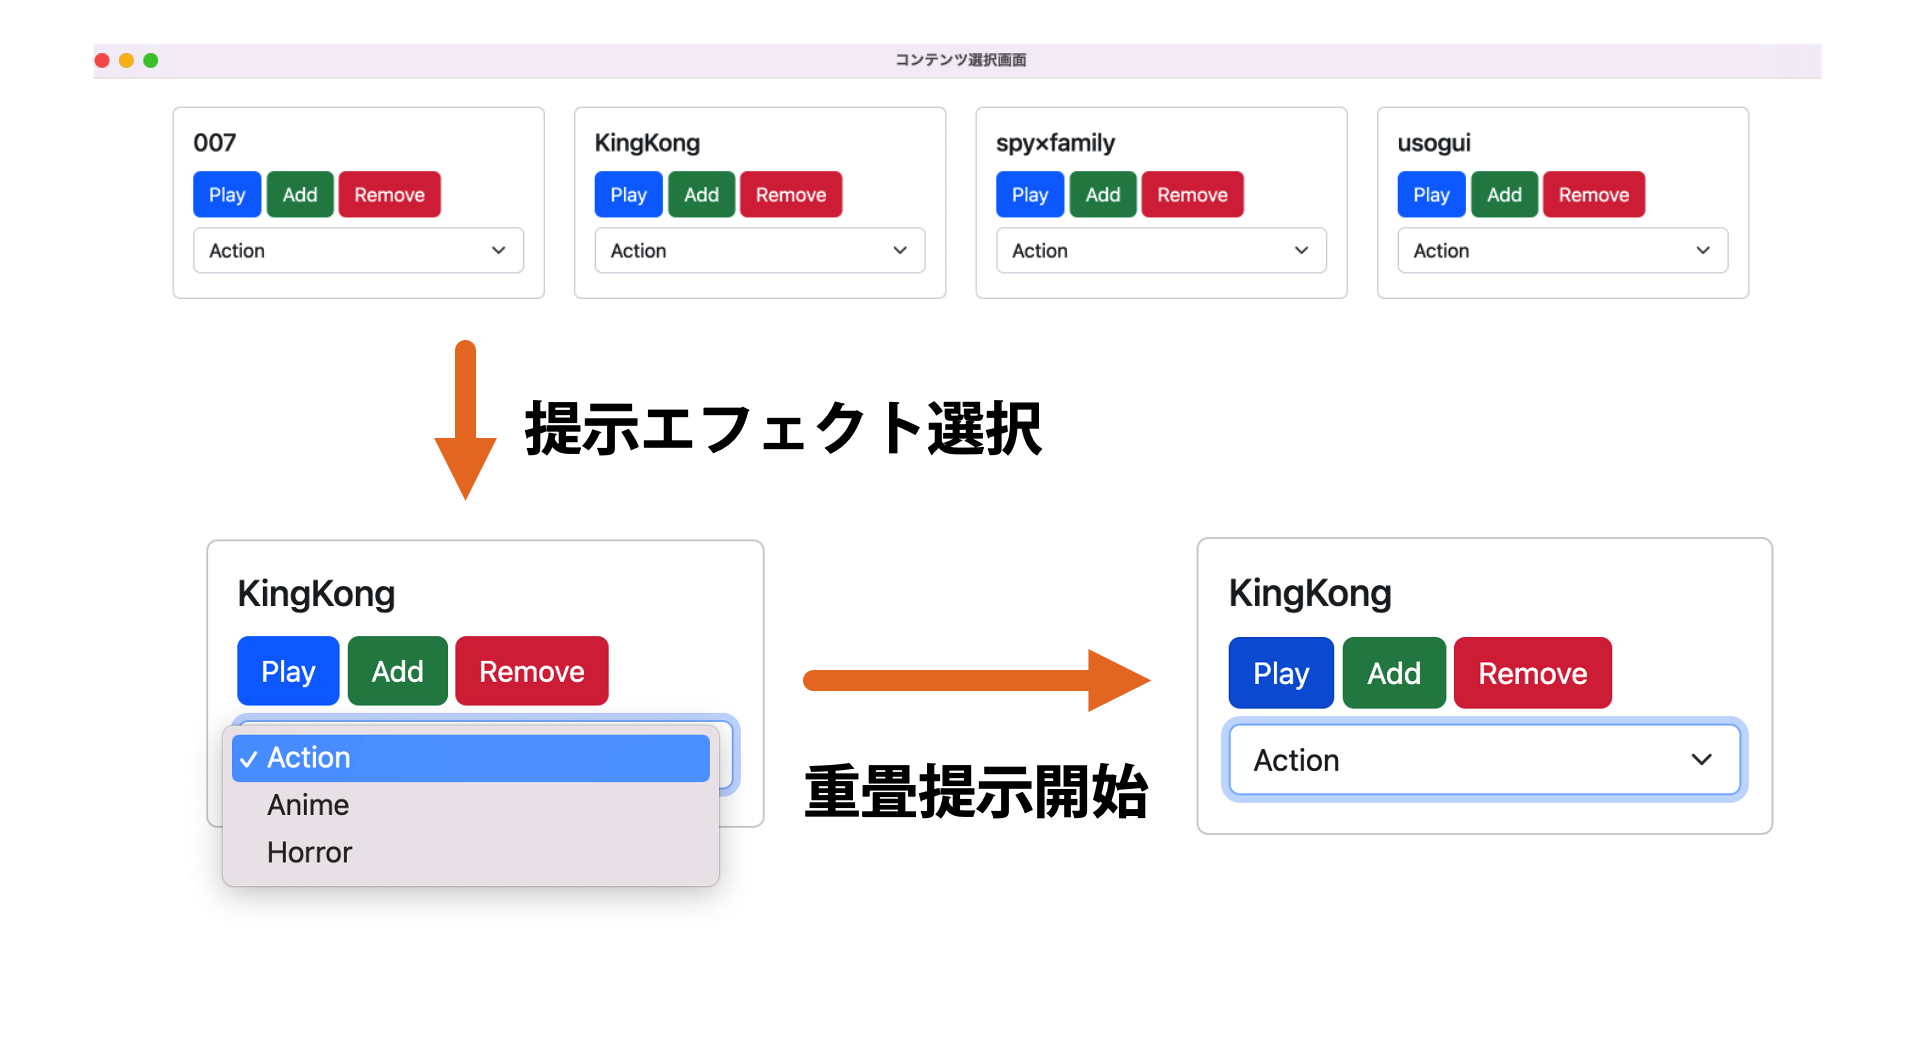
\includegraphics[width=17cm]{images/chapter3/efect_setumei.png}
   \caption{Electron動作画面(エフェクト提示選択)}
   \label{efectsentaku}
\end{figure}
 



\subsection{エフェクトの提示}\label{show_effect}

% レベルごとにエフェクト提示は、リアルタイムでデータ転送ができず、エフェクト制作の際にAfterEffectsを使用した為レベル分けを行なった。
% そのため、エフェクトをダイナミックに生成できず、細かな心拍数変化の表示ができていない。

エフェクトの提示として,表示するエフェクトを3種類に分け1種類に2つのエフェクトを制作した.
エフェクトを種類別に分けたのは,視聴する映画のジャンルを3種類(Action,Anime,Horror)に分け新しい視聴効果を引き出すためである.
エフェクトの目的として,Actionは迫力/緊迫感を与える,Animeはより面白さを与える,Horrorは恐怖感を軽減させるとして制作した.
エフェクト提示の実装画面を図\ref{efectteiji}に示す.
AfterEffectsの使用では透過TIFF書き出しを行う.
エフェクト提示の際に透過の範囲が決めやすく,エフェクト修正を即時変更可能であるため.
Actionのエフェクトは,迫力/緊迫感を与える目的のためノイズの赤色を画面の両淵に配置し,視聴に影響が出ないようにした.
制作方法としてAfteEffectsを使用し,フラクタルノイズ効果/色かぶり補正を使用した.
フラクタルノイズ効果はコントラスト60,明るさ0.0,複雑度6.0,展開1×+190.0,不透明度100とした.
色かぶり補正はブラックをマップのカラーを黒,ホワイトをマップのカラーを赤にした.エフェクトレベルが上がり,コントラストを60から80に上げて制作した.
評価実験を繰り返す中で,画面全体に赤色と黒色のぼかしエフェクト重畳で映像視聴に影響が出てしまい,
エフェクトに目が注視してしまい映画視聴がしずらい意見があったため画面の両端にエフェクトを配置し黒色のの歌詞をなくす修正をおこなった.
図\ref{actionbefore}にエフェクト修正前と修正後を示す.
Animeのエフェクトは,より面白さを与える目的のため漫画などで使用される効果線を画面全体に配置し視聴の邪魔にならずエフェクト効果を感じられるようにした.
 
制作方法としてIllustratorを使用し,ペンツールで塗りを白,線をなしにした.エフェクトレベルが上がり,白色の効果線の数を増やし,白の太さを太く,黒の効果線を増やす修正でエフェクト効果を感じられるようにした.
Horrorのエフェクトは,恐怖感を軽減させる目的のため画面全体に白のノイズをかぶせ映像を見やすくするようにした.制作方法としてAfteEffectsを使用し,フラクタルノイズ効果/色かぶり補正を使用した.
フラクタルノイズ効果はコントラスト50,明るさ0.0,複雑度3.0,展開1×+100.0,不透明度100とした.色かぶり補正はブラックをマップのカラーをなし,ホワイトをマップのカラーを白にした.
エフェクトレベルが上がり,コントラストを50から70に上げて制作した.
評価実験を繰り返す中で,画面全体に灰色のぼかしエフェクト重畳で映像視聴に影響が出てしまい,映像自体が見えなくなってしまう意見があったため画面中心を白くし周りを薄い白色でぼかす修正をおこなった.
図\ref{horrorbefore}にエフェクト修正前と修正後を示す.
 
\begin{figure}[H]
   \centering
   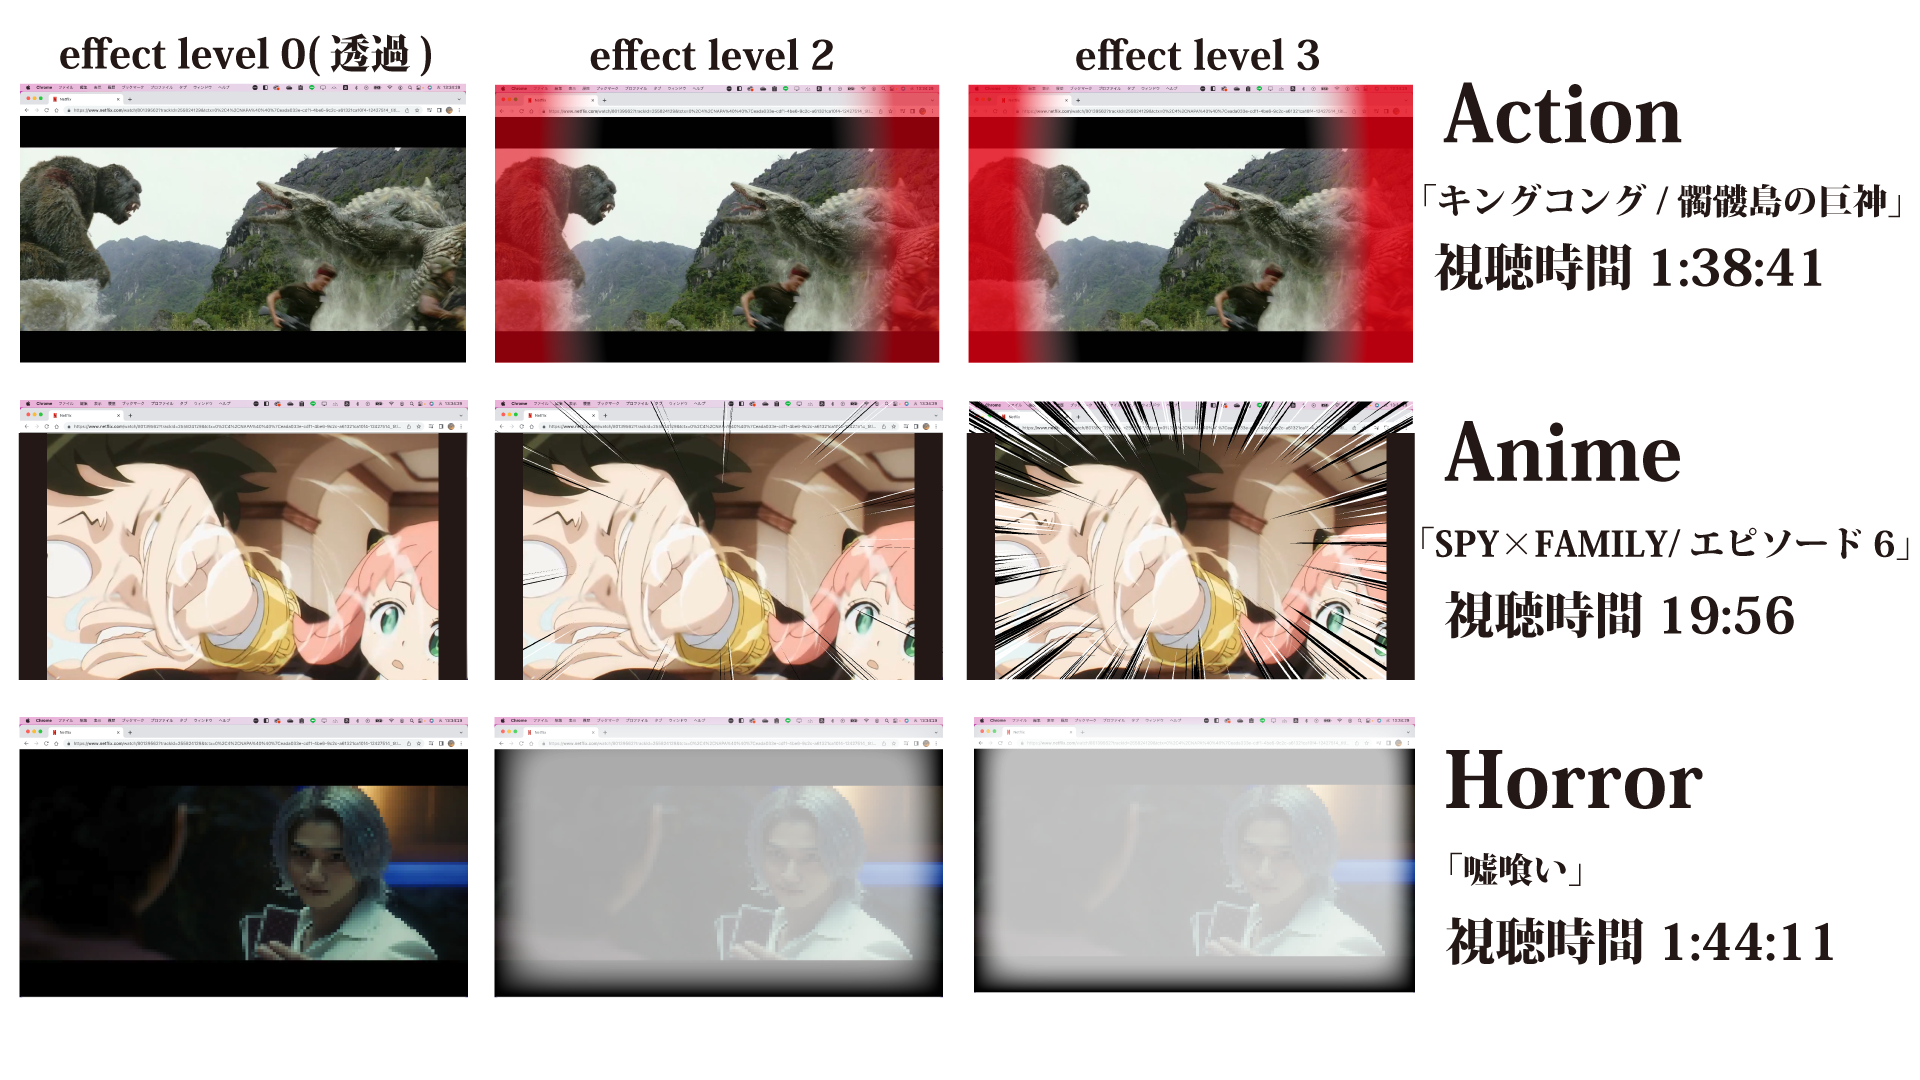
\includegraphics[width=16cm]{images/chapter3/efects.jpg}
   \caption{エフェクト提示画面}
   \label{efectteiji}
\end{figure}
 
\begin{figure}[H]
   \centering
   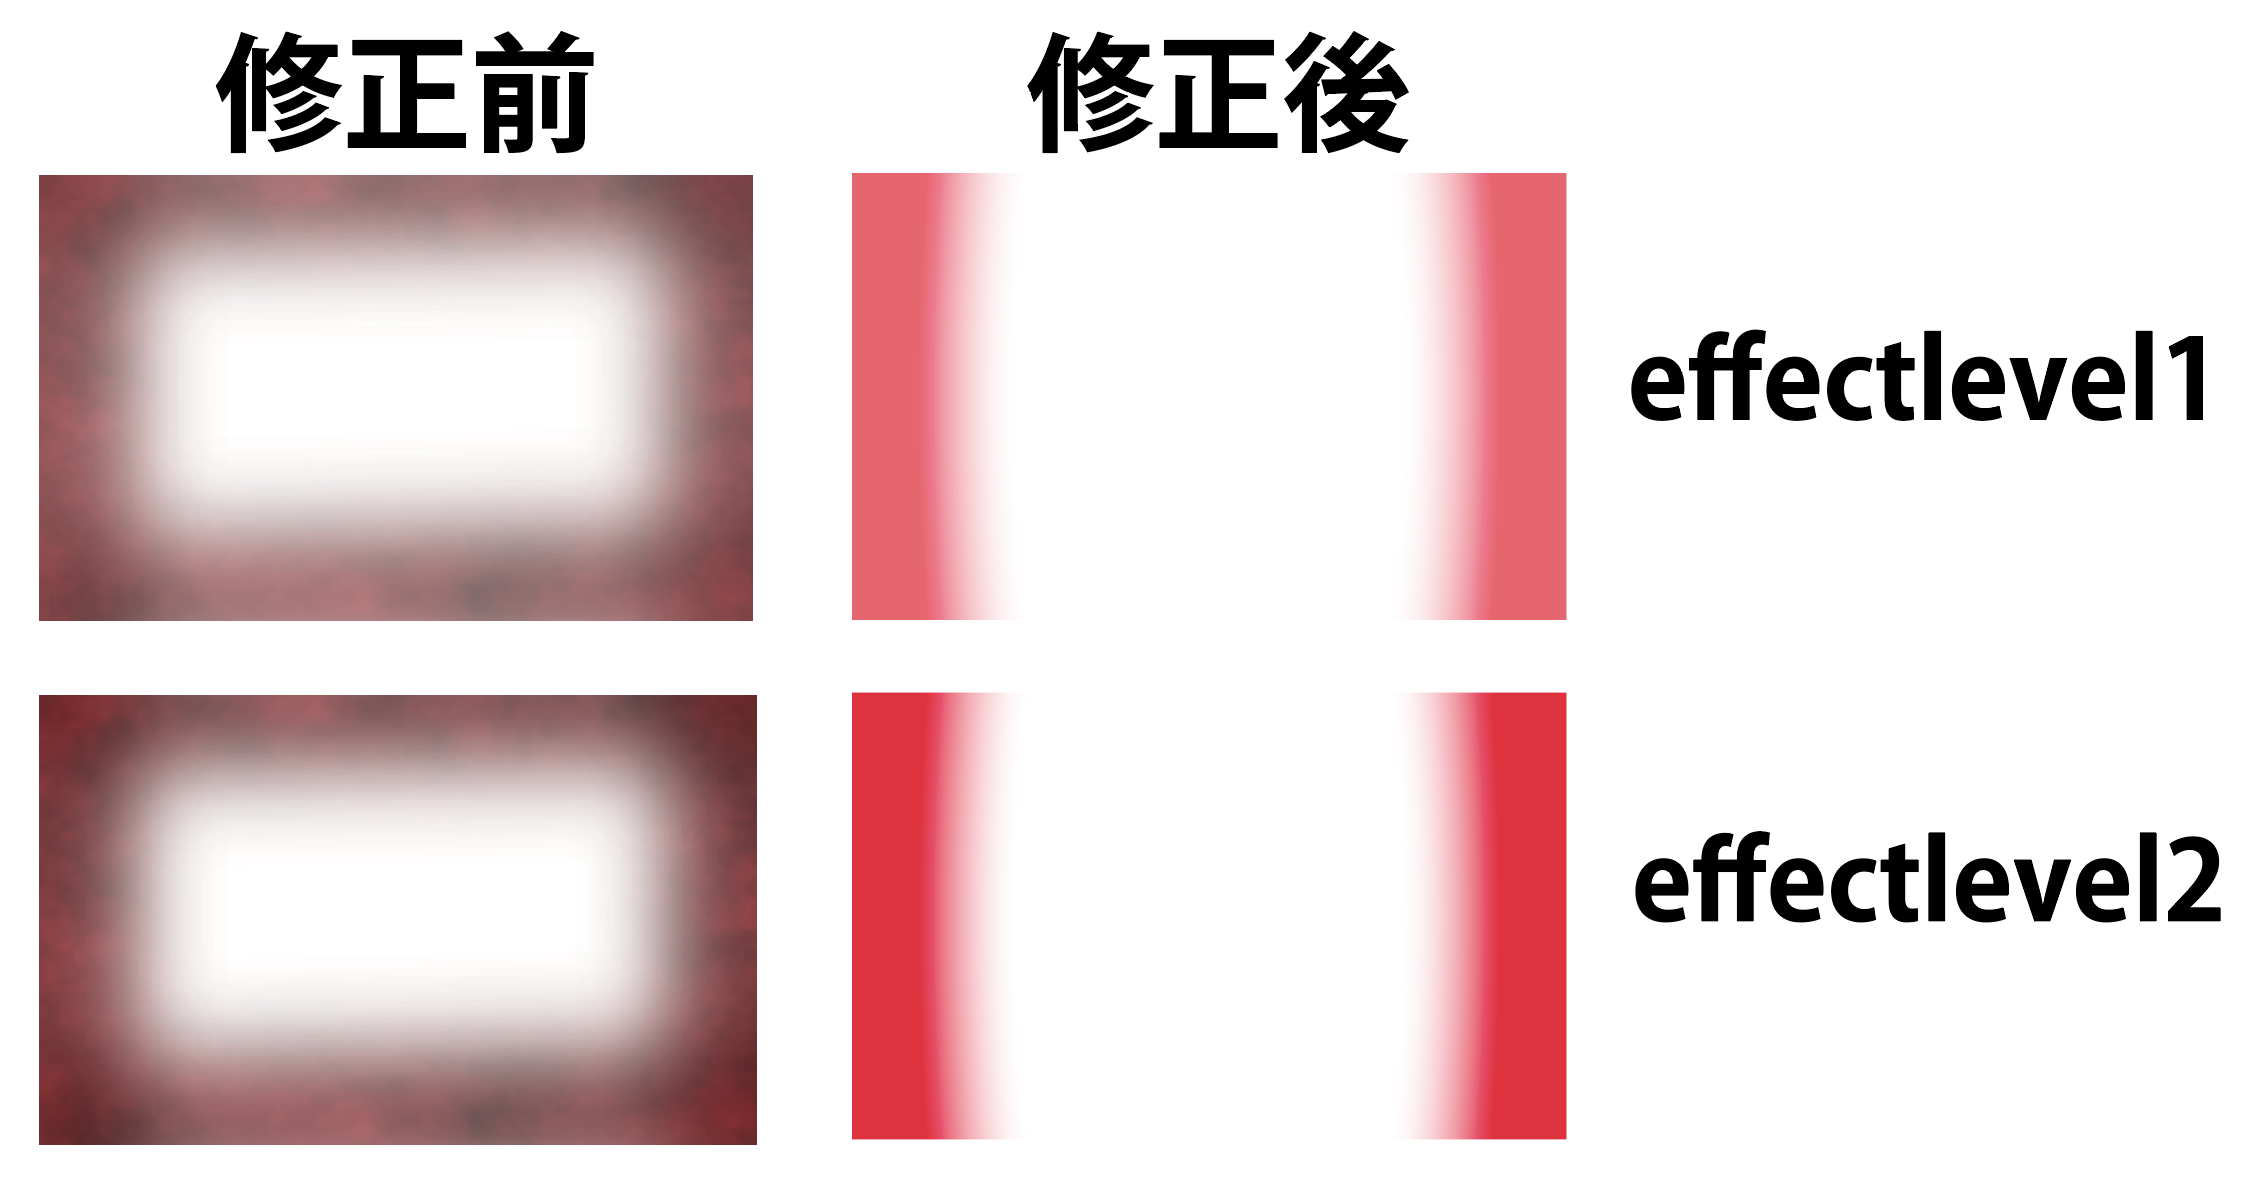
\includegraphics[width=16cm]{images/chapter3/actionberore.jpg}
   \caption{Actionエフェクトの修正}
   \label{actionbefore}
\end{figure}
 
\begin{figure}[H]
   \centering
   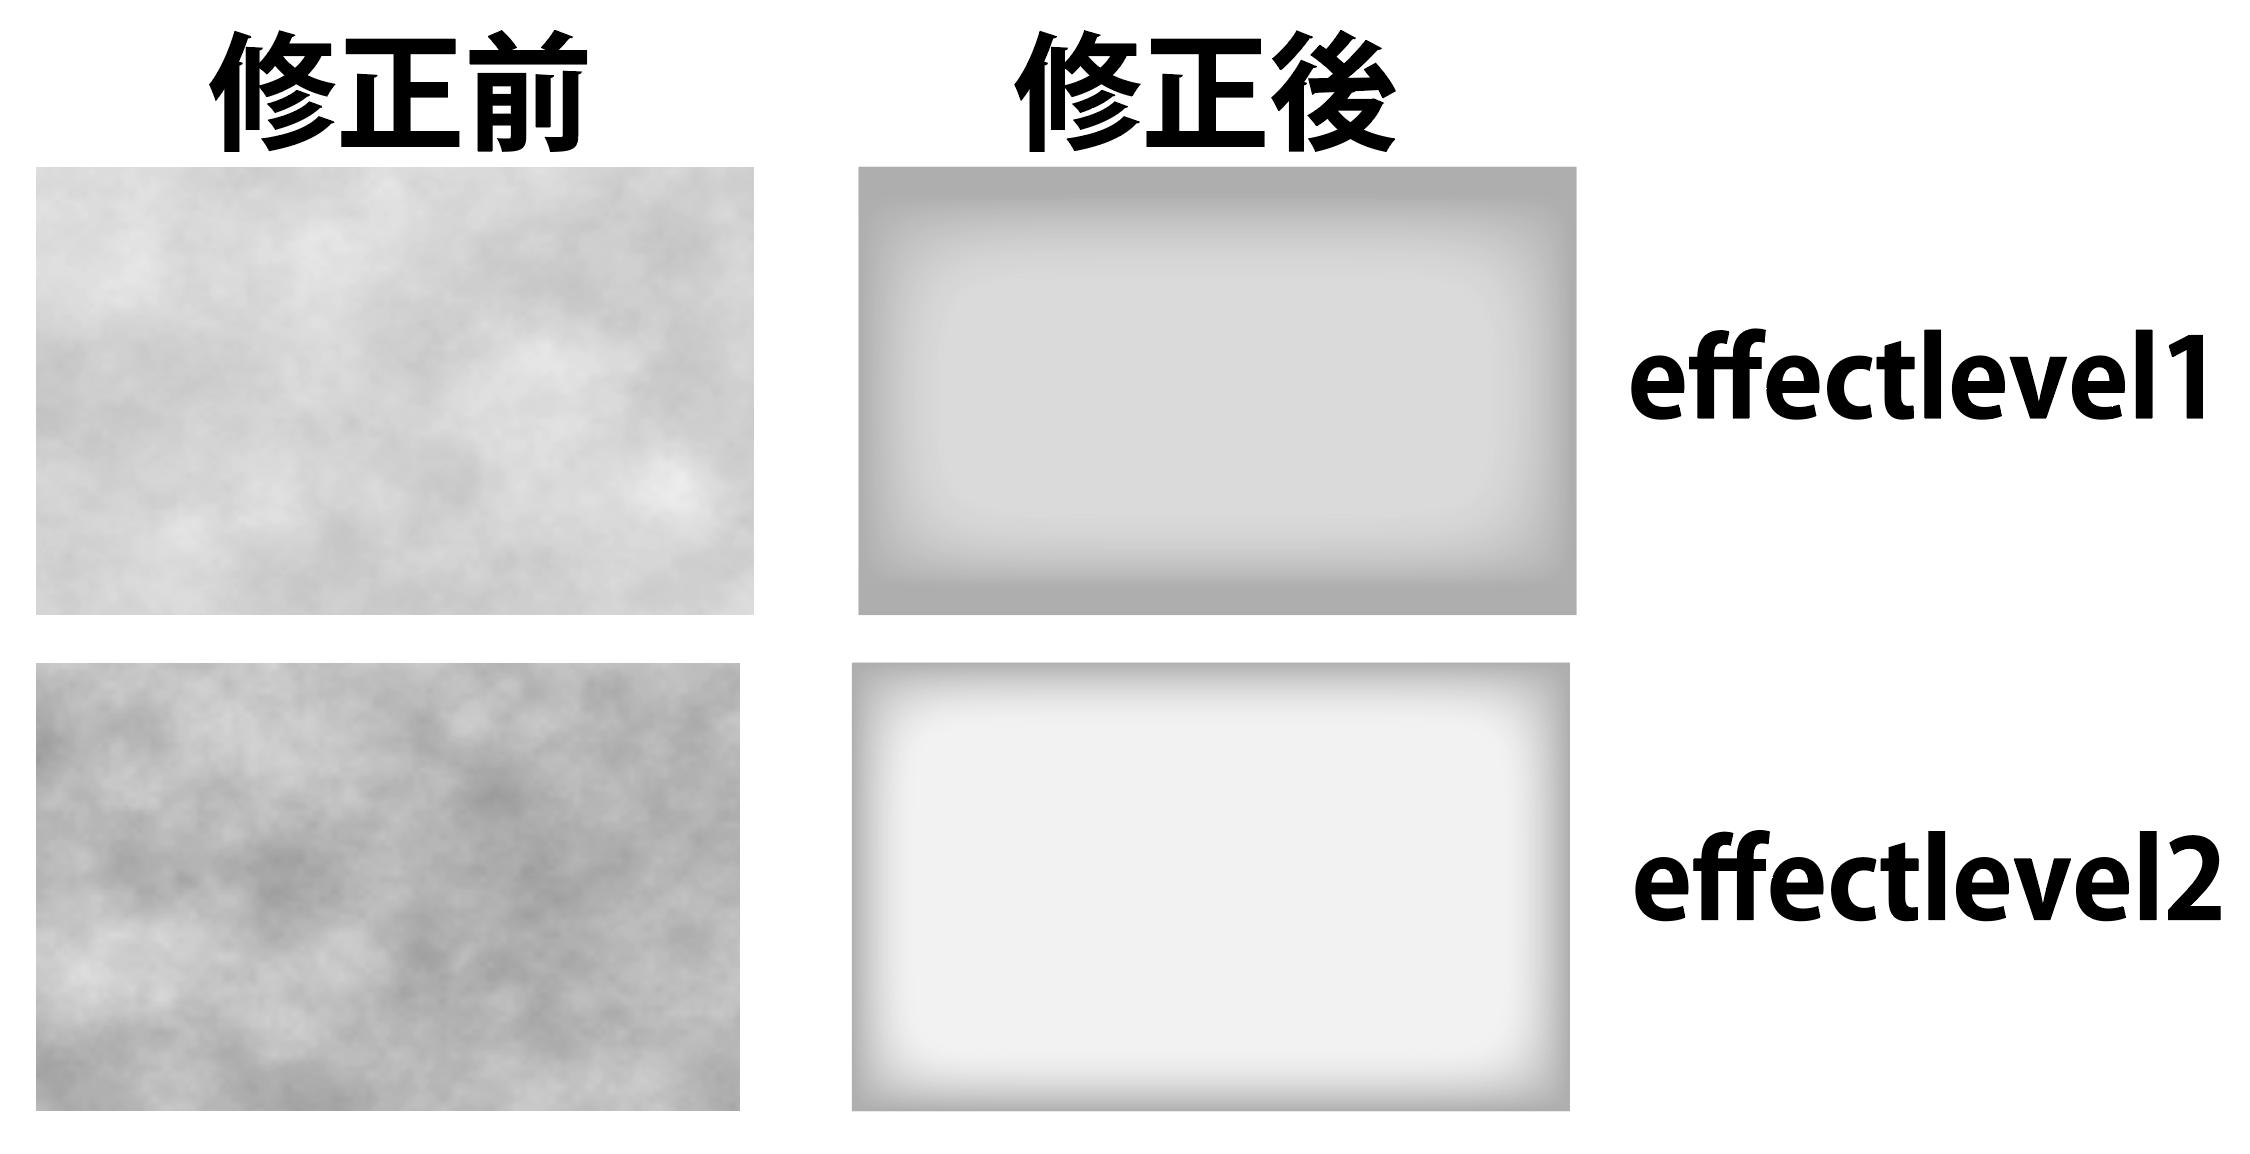
\includegraphics[width=16cm]{images/chapter3/horrorbefore.jpg}
   \caption{Horrorエフェクトの修正}
   \label{horrorbefore}
\end{figure}